\documentclass[preprint]{elsarticle} % Use elsarticle class (preprint option, no natbib options needed)

\usepackage[utf8]{inputenc} % Handle character encoding
\usepackage{amsmath, amssymb} % Mathematical symbols and fonts
\usepackage{graphicx} % For including graphics
\usepackage{hyperref} % For hyperlinks
\usepackage{natbib} % For citation management (uses natbib style)
\usepackage{booktabs}
\usepackage{wrapfig}
\usepackage{fancyhdr}
\usepackage{float} 

% Bibliography settings:
\bibliographystyle{elsarticle-harv} % Numeric citation style (you can change this if needed)

% Title and author info (you can adjust this to suit your paper)
\title{Variance in Environmental Mentions Across Constituencies in England}
\author{Kaley Burg}
\address{The University of Vienna}

\author{Martyn Egan}
\address{Trinity College Dublin}

% Customize the page style for this specific page
\fancypagestyle{special}{%
	\fancyhf{} % clear all header and footer fields
	\renewcommand{\headrulewidth}{0pt} % remove header line
	\renewcommand{\footrulewidth}{0pt} % remove footer line
	\fancyfoot[R]{\thepage} % put the page number on the right side in the footer
}


\begin{document}
	
	\begin{abstract}
		This study measures the variation of leaflet campaign messages by constituency in England within each major political party (Conservative, Labour, Liberal Democrats, Green, and UK Independence) during the 2010, 2015, 2017, and 2019 General UK Elections. This is done using leaflet data from OpenElections \citep{milazzo2020openelections}. The text from each leaflet is scraped and analysed with the Laver \& Garry Quanteda dictionary \citep{laverEstimatingPolicyPositions2000} on policy positions with frequencies of environmental or climate mentions counted for each constituency by year and political party. These are compared to the other constituencies belonging to the same party. Variance among constituencies in environmental mentions is compared to weather data in England as well as previous election voteshare and 2011 census data regarding income, age, and education level of citizens within the constituencies. The aim of this study is to determine the frequencies of topic mentions and identify factors which are most strongly related to these changes in frequency in local politician campaigns in UK general elections.
		

	\end{abstract}
	
	\maketitle % Prints the title page
				
	\newpage
	
	\section{Introduction}
	
Issue salience within party manifestos in England can be used to shed light on both the current political climate as well as the major goals and priorities of a political party. For instance, past research has shown that different parties consistently highlight different issues, such as the Labour Party with employment, the Conservative Party with law and order and rural life, and the Liberal Democrats with the environment \citep{pogorelisIssueSalienceRegional2005}. Beyond variance in messaging and campaigning between the political parties, variance exists within parties themselves. Within political parties in the United Kingdom, the amount of campaigning done and resources utilised is determined by constituency resources (rather than whole party resources) and incumbency status within the constituency that the campaign takes place \citep{pattieIncumbentPartiesIncumbent2017a}. This demonstrates the need to understand party campaigns on the constituency level in order to capture and understand the current political sphere.


This also relates to political geography, such that political behaviour is geographical and has implications on the voting habits as well as campaign messages. This has been studied within different regions in Scotland, finding that there is variation of campaign strategies within political parties depending on the location of the campaign \citep{pringleClassicsHumanGeography2003,agasosterPartyCohesionLocal2001}. Campaign strategies can pertain to both messages within campaigns as well as the number or frequency of campaigns in specific areas. Regarding campaign messaging, election leaflets are often looked at as they continue to serve as the most common way of campaigning. Variation has been found within these leaflets, specifically in the 2019 UK General Election, as mentions of specific issues or parties is not consistent throughout all constituencies in England  \citep{trummParliamentaryCandidatesTheir2023a}. Not only is there variance in mentioned issues and topics within leaflets, but also the distribution of these leaflets may not be uniform, as campaigning in constituencies may also vary due to campaign funding itself, with target seats emphasized and focused on more in campaign strategies \citep{pattieResourcingConstituencyCampaign2016}. This is in part influenced by the distribution of the electorate, as major political parties aim to reduce abstention and third parties aim to sway voters away from the main two parties \citep{nunezEffectsLocalCampaigning2021}.

Issue salience generally has typically been focused on different parties as a whole. For example, Green parties have the highest environmental issue salience, social democratic parties tend to have higher environmental salience than conservative parties, and parties on the left have higher environmental salience overall because they are in more competition for votes with the Green Party \citep{carterGreeningMainstreamParty2013}. The tendency of parties to mention the environment is also influenced by public opinion \citep{carterPartyPoliticizationEnvironment2006}. There has been limited research, however, on issue salience within parties by constituency. Local campaigns do vary based on constituency in the issues that are mentioned, specifically with Conservatives and Liberal Democrats mentioning issues that are not stated in their overall manifestos \citep{harrisonNationalLocalParty2008}. This study by Harrison and McSweeney highlights the basis of this dissertation: there is variation in the issues mentioned within UK campaign leaflets. The first goal of my research is to add to this body of work by determining not only how the content varies between constituencies but how these content mentions vary in \textit{frequency} throughout UK constituencies.


As the goal of campaigning is success in both the local campaign and on a national scale, party campaign success should be examined as well. While greater campaign efforts within a party typically result in better vote share, results are also impacted by the the strength of competitor parties as well as the incumbent party at the time of the election \citep{pattieIncumbentPartiesIncumbent2017a}. For this reason, it is important to understand which party constituencies typically vote for (and which issues they represent) in order to also understand how future politicians choose to campaign. Issue salience can be a useful indicator of campaign strategy as opposed to stance on the issue alone, as parties will mention issues more often if they expect to attract voters this way \citep{pogorelisIssueSalienceRegional2005}. While past literature on topic variance in campaigning has shown the mere presence of variance, it does not explain why this variance is present. Analysing correlating factors with issue salience variance may shed light on the rationale behind the strategies used by political parties in campaigns. The second goal of this dissertation is therefore to understand which factors are related to varying frequencies of topic mentions. 



\section{Literature Review}

\subsection{Public Opinion and Political Communication}

To understand the reason behind variation within political parties, it is important to first understand how these campaigns are broadly created. Parties are attentive to changes in voter opinions, such that they dedicate resources to telephone, door-to-door, and email canvassing of members of the electorate in order to develop their campaigns \citep{fisherFootsloggingCallCentres2008}. Furthermore, parties have the capacity to respond to new information about public opinion in order to improve their campaigns \citep{hartmanLearningJobAdapting2017}. The type of public opinion matters though, as European parties tend to change their campaigns in response to public opinion that clearly denotes a shift in public opinion away from the party, rather than changing their campaigns due to more general public opinion shifts \citep{adamsUnderstandingChangeStability2004}. 

Mention of specific topics, such as the environment and climate change, in campaigns and manifestos is also determined in large part by where issues fall on the classic left/right divide \citep{farstadWhatExplainsVariation2018}. Public opinion and party alliance are interconnected as well though, as research, especially in the USA, has demonstrated that both political elites and general citizens associated with Republican/right-leaning parties tend to be more dismissive of the existence of climate change  \citep{dunlapPoliticalDivideClimate2016,mccrightPoliticizationClimateChange2011}. This demonstrates that a party may continue to highlight issues associated with their political side until there is both a shift in public opinion on the topic as well as an opposing side party that is highlighting the topic \citep{carterPartyPoliticizationEnvironment2006}. In constituencies where support for a specific party is and historically has been high, then they therefore may not be pushed to incorporate issues into their campaign that are historically not associated with their party. 

Issues may be pushed within a party when a rival party threatens an incumbent one. Regardless of whether it has an impact on the effectiveness of a campaign, an incumbent party may campaign harder when threatened by a challenger party in the constituency \citep{pattieIncumbentPartiesIncumbent2017a}. This introduces vote share of previous elections (as well as public opinion) as a feature of importance in determining which factors may prove to be the most useful in understanding variance in the frequency of environmental mentions in election leaflets.


\subsection{Factors Influencing Public Opinion}

\subsubsection{Weather Events and Climate Attitudes}

As public opinion may be important in understanding where and why variation may occur in campaign strategies throughout constituencies, it is therefore important to also identify factors involved in the formation of these opinions. Specifically, as this study will focus on environmental mentions, formation of attitudes regarding climate change and environmental issues of the general public may provide useful insight. Although past research has found little to no association between experiencing climate extremes and changes in climate change opinions, \citet{koniskyExtremeWeatherEvents2016} found that, with more specific geospatial resolution, extreme weather events in the last month (or several months for more extreme events) does increase concern about climate change. This study also found that ideology and partisanship have an impact on these attitudes \citep{koniskyExtremeWeatherEvents2016}. 

Other forms of climate events may affect public climate opinions as well. \citet{viscontiEffectDifferentExtreme2024} found that in the US, floods and storms did not seem to have an effect on climate attitudes. This was also supported by \citet{loComeRainShine2015}, who found that individuals may not attribute increased rainfall or flooding to climate change, meaning that different weather events may have different effects on climate beliefs. Intricacy in observing weather patterns on their own is complex as well, such that physical and psychological proximity to a natural disaster may differ, meaning that those nearby an events but are not directly affected may have different belief outcomes than those that are nearby \textit{and} directly affected \citep{siscoEffectsWeatherExperiences2021}. Furthermore, individuals may not perceive changes in temperature accurately, thereby making it difficult to assess climate attitudes based on temperature changes alone \citep{goebbertWeatherClimateWorldviews2012}. However, the same study by \citet{goebbertWeatherClimateWorldviews2012} found that rainfall and soil moisture are closely related to actual data on flooding and drought, but the perceptions surrounding these events are influenced by ideological and cultural factors pertaining to individuals experiencing them, which is in line with research from \citet{osberghausNaturalDisastersClimate2022} as well.

Although some studies have shown that proximity to natural disasters is crucial to changing climate beliefs, \citet{albrightBeliefsClimateChange2019} found that direct experience with flood damage is less important as time goes on and that what is more impactful is the perception of community damage and safety from natural disasters. In the case of election campaigns, this may have an impact on campaigning as politicians may be gauging the public perception of climate change over a longer period than just the time period directly after a flood or natural disaster. Regarding the mechanisms behind these changes in opinion, attribution of flooding and other events to climate change itself is an important element to consider. Similar to how \citet{loComeRainShine2015} found that different weather events may be associated with different perceptions of climate change, the same event, such as a flood, may or may not be attributed to climate change based on whether an individual is directly affected by the event, with the effect moderated by political party affiliation \citep{ogunbodeIndividualLocalFlooding2020}. Political party affiliation or preference may be inversely affected by climate events as well, specifically when implicit or automatic associations towards politicians and policies is measured instead of explicitly stated attitudes \citep{rudmanWhenTruthPersonally2013a}. 

In addition to just changing beliefs in climate change overall, individuals may support different electricity or energy policies that may not be inherently tied to their climate beliefs. For instance, \citet{osberghausCausalEffectFlood2019} found that damage to an individual may not be inherently tied to support for green electricity as different households and communities may vary by income and eligibility for disaster relief, thereby producing differences in support for these policies. Furthermore, exposure to extreme temperatures in the UK was shown to have a statistically significant effect on concern towards energy security \citep{larcomUKSummerHeatwave2019a}. As politicians are inherently concerned with support for policies and parties, it may therefore be important to analyse factors that may be related to changes in environmental policy support even if they are not directly related to changes in climate change belief. 



\subsubsection{Other Correlates of Voting Behaviours}

\paragraph{Rural vs. Urban Constituencies}

Throughout Europe, political views tend to vary depending on location, such that those living outside of cities tend to be more conservative but more active about voting, whereas those within cities may vote less often but engage in other forms of political demonstration \citep{kennyUrbanruralPolarisationPolitical2021}. Urban and rural areas also differ significantly in terms of the demographics of those who live in each area. \citet{patemanRuralUrbanAreas2011} discusses differences between both rural and urban areas as well as sparse/isolated vs non-sparse areas: for instance that rural non-sparse areas have the lowest levels of poverty, that young adults tend to move to urban areas from rural areas, and rural areas tend to have a lower crime rate than urban ones. These factors may also play a role in the type of issues that candidates may focus on in their campaigns. These areas may have different political precedents due to differences historically, especially regarding the internet as there was previously a divide in access to internet between rural and urban areas, as found by \citet{choudrieRealisingGovernmentUK2005}. However \citet{patemanRuralUrbanAreas2011} found current equal access to the internet, with rural areas sometimes having greater access than urban areas.

In terms of environmental issues specifically, \citet{bognerEnvironmentalPerceptionRural1997} found little to no difference between rural and urban students regarding environmental attitudes and behaviours. This finding has been confirmed in more recent work as well, with the perspective instead being that measurement tools surrounding attitudes and behaviours should be more inclusive for both urban and rural behaviours to allow for more accurate comparison \citep{huddart-kennedyRuralUrbanDifferencesEnvironmental2009}. Although concern towards the environment as it has typically been measured appears to be higher in urban areas, differences seemingly arise more from different types of environmental concern between rural and urban individuals \citep{deberenguerRuralUrbanDifferencesEnvironmental2005}. Although the difference does not seem to lie in overall differences between rural and urban-dwellers, the form in which their environmental concern may take may have impacts for policy-makers. \citet{freudenburgRuralUrbanDifferencesEnvironmental1991} suggests that policy-making may be nuanced in rural areas, as farmers and other groups may be less inclined to engage in environmental behaviour regardless of expressing pro-environment attitudes and policy-makers may similarly appear pro-environmental without suggesting any specific environmental policies. This provides more reasoning to view environmental mentions in campaigns on a quantitative scale rather than a binary scale, in order to hopefully obtain an indicator of how seriously environmental issues are seen.

\paragraph{Remaining Demographic Factors}

In isolating other factors that might be related to environmental concern, many authors have found it difficult to find straightforward relationships between demographic factors (such as socioeconomic status, political views, etc.) and environmental concern \citep{dietzSocialStructuralSocial1998,samdahlSocialDeterminantsEnvironmental1989,giffordPersonalSocialFactors2014}. The issue in finding a relationship may however be more related to the wording of questionnaire items used to measure environmental concern. \citet{klinebergDemographicPredictorsEnvironmental1998} found that younger and more educated individuals tend to express greater environmental concern regardless of measurement differences, while the effects of other demographic factors on concern level depend heavily on how questions are worded. Whether age is a good predictor of environmental concern is also relatively contested in the literature, with some findings showing age to be a more significant factor than education \citep{buttelAgeEnvironmentalConcern1979}, with later research suggesting that environmental education is increasing across the population, making education the driving factor of environmental concern \citep{howellChangingFaceEnvironmental1992}. Education and age together being a predictor of environmental concern has also been found in some research \citep{arcuryEnvironmentalWorldviewResponse1990}, in addition to other factors such as income \citep{gambaFactorsInfluencingCommunity1994} and political ideology \citep{dunlapImpactPoliticalOrientation1975}. As the scope of this study extends to the constituency level and is less concerned with individual opinions towards the environment, it would seem that regardless of \textit{how} these various demographic predictors (age, income, education, and political orientation) are related to environmental and climate attitudes, that politicians may still be taking these factors into account in their campaign strategies.

This study aims to find the underlying mechanisms behind politician campaign strategies across constituencies. Although politician motivations are not included as a focus in this study, this research will instead provide information on which factors across constituencies have the ability to influence campaigns. The expected results are therefore that political party will not be the sole driving factor behind these differences, and instead the relationship may be much more complex. 
	
	
	\newpage
	

	
	\section{Data and Methods}

The outcome data will be measured using leaflet data from OpenElections \citep{milazzo2020openelections}. This contains information from the 2010, 2015, 2017, and 2019 UK General Elections, with leaflets uploaded and coded based on constituency, party, issues mentioned, etc. The OpenElections data contains images of the leaflets as well as the metadata obtained by human coders. In order to enhance this dataset and separate it from other previously existing datasets, this project will also use text-scraping from image techniques. \citep{KerasocrKeras_ocrDocumentation,hoffstaetterPytesseractPythontesseractPython}. This process involves machine learning algorithms that detect text from an image and uses Optical Character Recognition (OCR) \citep{madhugiriExtractTextImages2022}. This will be supplemented with Pytesseract's text orientation function that detects both the language of the text as well as if the text is rotated \citep{rosebrockCorrectingTextOrientation2022} in order to be able to flip the images that are rotated either 90 or 270 degrees. As there were over 18,000 images scraped from the OpenElections website, this step will be crucial in order to ensure that the highest possible amount of text is preserved. Due to the high computational needs of this project, Trinity College Dublin's Callan cluster will be used to process the images using batch jobs.



The text will then be sorted using the Laver Garry dictionary \citep{laverEstimatingPolicyPositions2000} with frequencies of each category of words counted for each constituency, party, and year. The words pertaining to the environment from this dictionary are divided into pro-environment words (ie., "car", "chemical", "ecolog", "emission", "green", "planet", and "product") as well as con-environment words (ie., "product"). In addition to these words, I will add a 'climate' subcategory consisting of the following words: "climate", "climate change", "global warming", "carbon emissions", and "greenhouse gases." These words were selected by reading through several leaflets and finding common words pertaining to the environment in order to best match the definition of environmentally related words to the human coders. Once the dictionary is used and the leaflets' text is divided into cleaned tokens, the environment (among the others) subcategories will be condensed together and the number of words matching in any of the subcategories will be counted and stored as a count variable in the dataset. This dataset therefore will not take into account the type of environmental mentions included in the leaflets, although this could be an avenue for further research. 

Furthermore, as this project will use text scraped from leaflets rather than articles or speeches, the pre-processing of the text will follow a slightly different approach than standard text analysis projects. Rather than removing stop words and finding collocations, the data cleaning process will minimally process text data, primarily removing symbols and numbers. As the text is not necessarily in the correct order, this will be necessary to make sure that the analysis does not miss any important mentions. The text data obtained from this process will then be compared back to the metadata that was created by human coders but will also be used to examine issue salience and frequency of mentions beyond what can be done with human coders \citep{trummParliamentaryCandidatesTheir2023a}. The metadata for the leaflets only contains a binary measure of mentions: either the leaflet mentions the issue or it does not. Although this will be useful for ensuring accuracy of the keras-OCR model, it does little in capturing a full image of fine details in campaigns. 
 


After the text has been scraped, variation within each topic will be measured between constituencies as well as between each party and election year. Data from Meteostat \citep{MeteostatPyPI} will be used to collect weekly weather data from one year before the election date to the election date. This time period was chosen based on past literature suggesting that extreme weather events are most salient closer to the event \citep{viscontiEffectDifferentExtreme2024}.The data will then be converted into a single variation variable, through taking the standard deviation of the aggregate weather data as a single measure of how inconsistent the weather is at each location and to measure any major changes that might be salient to those living there. This is to obtain a general summary of how weather patterns vary across the UK in the year leading up to each election.


\paragraph{Controls}

In addition to weather data, various demographic factors will be used as controls. Control data will be taken from the 2011 UK Census \citep{2011CensusOffice}, as this is the nearest census data to all of the elections in the dataset (2010, 2015, 2017, and 2019) as the 2021 census was not released yet. These controls will include median age, proportions of individuals with various educational attainment, and average income. In order to use educational attainment, the total number of students, regardless of employment status, will be summed to collect a total number of students within a constituency. As income data is not readily available numerically in the 2011 census, occupational rank will be used in its place. These overarching categories are: Higher managerial, administrative and professional occupations, Large employers and higher managerial and administrative occupations, Higher professional occupations, Lower managerial, administrative and professional occupations, Intermediate occupations, Small employers and own account workers, Lower supervisory and technical occupations, Semi-routine occupations, Routine occupations, Never worked, Long-term unemployed, and Full-time students. These are pooled across both males and females and are included as count variables in the dataset.

Data on rural or urban classification of each constituency will also be used from the 2011 Rural Urban Classification of Westminster Parliamentary Constituencies \citep{RuralUrbanClassification}, focusing on the total rural/urban population count in each constituency, as well as voteshare data \citep{watsonGeneralElectionResults2024}. The voteshare data includes vote count and vote share from 1918 to 2019 but will be subset to include just data for the 2010 to 2019. This will be used as an indicator of the party competition for each election year within constituencies. As the constituency boundaries changed in 2010 \citep{cracknell2010GeneralElection2024}, the analysis will focus just on the party competition for each election as opposed to political leaning of the constituency in past elections as well. An analysis of changes in vote share for each of the parties in England could provide a useful avenue for future research on this topic. 

To ensure that the model is not picking up changes based on political party alone, a two-way fixed effect model with both election year and constituency as fixed effects will be run first. If the expected result is observed, this model should should very little significance of political party in capturing the overall variance, with most variance presenting in the constituency factors themselves.

Next, constituency as a fixed effect will be removed, leaving election year as a single fixed effect. In line with the primary hypothesis, this model is expected to be the most useful in determining what is causing variance across constituencies, while also controlling for variance that would be natural expected from election to election. The need for both models are to first demonstrate that political party cannot be used as a sole explainer of variance across constituencies in their mentions of environmental mentions and that it is important to look deeper into the constituency-specific factors that instead impact local campaigning.
	
\newpage

\section{Models and Results}


\subsection{Descriptive Statistics}


The text scraping accuracy results for environmental mentions is shown in Table~ \ref{tab:envaccuracy}. The first accuracy score of 88.66\% means that for every time the metadata lists the environment as a mentioned issue, the OCR text-scraping methods also find at least 1 mention of an environmental-related word approximately 89\% of the time. This accuracy score, in the scope of this project, shows that the machine learning OCR method used to scrape the text, as well as the dictionary used, has an accuracy of almost 90\%. This is considerably good given the large volume of data and automated text-scraping methods on leaflets that vary in image quality.

The second accuracy score describes the frequency at which the metadata that was scraped from the OpenElections website lists the environment as one of the mentions during conditions in which the leaflet text that I scraped \textit{also} shows some mention of the environment. The score of 58.07\% indicates that, assuming my text-scraping methods are correct, the human coders only catch environmental mentions approximately 58.07\% of the time. 




\vspace{0.5cm}


\begin{table}[!htbp]  
	\caption{Accuracy of Text-Scraping Methods on Environmental Issues} 
	\label{tab:envaccuracy} 
	\begin{tabular}{|l|r|r|r|}
		\hline
		Condition & Count & Total & Accuracy \\ 
		\hline
		Accuracy of OCR detection when 'Environment' is in metadata & 2417 & 2726 & 88.66\% \\
		Accuracy of 'Environment' in metadata when OCR detects mentions & 2417 & 4162 & 58.07\% \\
		\hline
	\end{tabular}
\end{table}



\vspace{0.5cm}

As a robustness check to ensure that these results extend to the rest of the dataset, Table~\ref{tab:econaccuracy} displays the accuracy results for economy mentions as well. This table displays interesting results, such that the OCR methods used in tandem with the Laver Garry dictionary \citep{laverEstimatingPolicyPositions2000} to detect mentions of the economy are accurate in almost 100\% of the cases where the human-coded metadata shows an economic mention in the leaflet. 

Both Table~\ref{tab:econaccuracy} and Table~\ref{tab:envaccuracy} demonstrate a discrepancy in the human coded data versus the text scraped from the leaflet. It appears that in cases of both environmental and economic mentions that the OCR method detects more mentions of both topics. However, the accuracy score is quite high for detecting what has already been picked up by human coders. This would imply that the combination of the text scraping and the use of the Laver Garry dictionary is able to go beyond what is possible with human coders alone. Furthermore, this method could also be used in a further analysis to look at which words in each category specifically are used most frequently throughout the leaflets. 


\vspace{1cm}

\begin{table}[!htbp] 
	\caption{Accuracy of Text-Scraping Methods on Economic Issues} 
	\label{tab:econaccuracy} 
	\begin{tabular}{lrrl}
		\toprule
		Condition & Count & Total & Accuracy \\
		\midrule
		Accuracy of OCR detection when 'Economy' is in metadata & 5322 & 5373 & 99.05\% \\
		Accuracy of 'Economy' in metadata when OCR detects mentions & 5322 & 7073 & 75.24\% \\
		\bottomrule
	\end{tabular}\\
\end{table}


\vspace{1cm}





% Include the image with text wrapping
\begin{wrapfigure}{l}{0.58\textwidth} % 'l' for left alignment, 0.58 of the text width
	\centering
	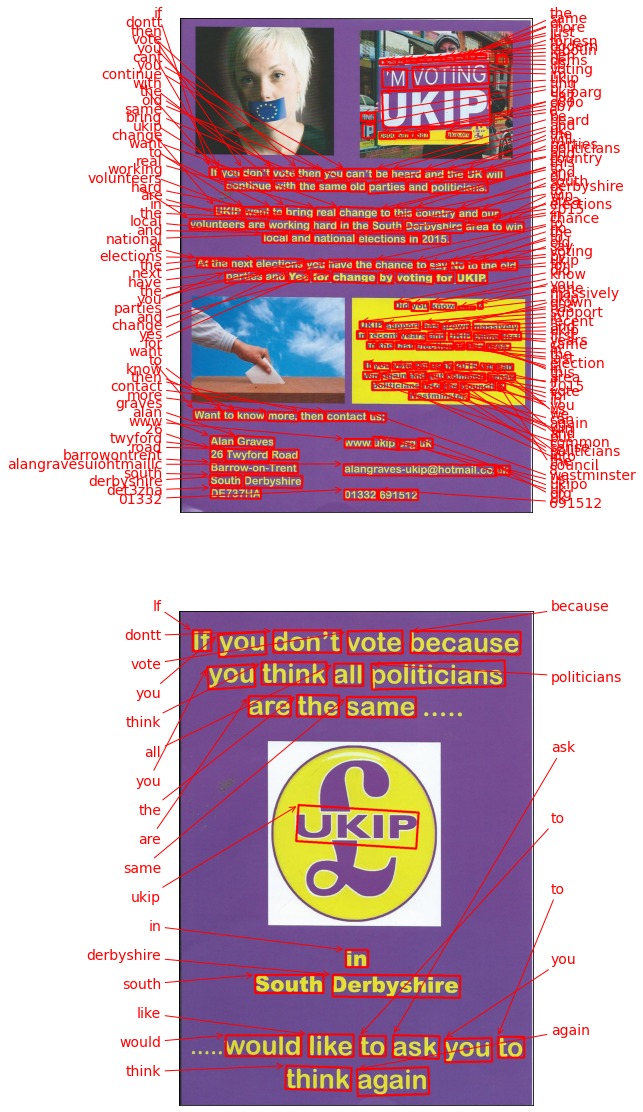
\includegraphics[width=0.58\textwidth]{ukip_example.png}
	\caption{OCR Method on UKIP Example}
	\label{fig:ukip_example}
\end{wrapfigure}


%%


One possible explanation for the variation between the accuracy levels regarding environmental mentions is that the human coders have inaccurately labeled the leaflets as having environmental mentions when none are actually mentioned. An example of this is in Figure~\ref{fig:ukip_example}\footnote{The unmarked leaflet is shown in the appendix for greater legibility}, where the metadata did include the environment as a mentioned topic, but the OCR method does not detect any mentions of the environment. Upon closer examination, it appears that the OCR method performs relatively well and that there does not seem to be any mention of the environment in either of the images pertaining to that leaflet. This further confirms that the OCR text-scraping method is robust enough to use for later analysis of variation among environmental mentions. 


Additionally, it is unclear exactly how the human coders are deciding which categories are mentioned in the leaflets. The OpenElection website allows any site visitor to upload or code a leaflet based on mentions and issues in the images. This introduces a great amount of variation in how the leaflets are potentially classified, as individuals may vary in their knowledge of politics or individuals may not detect all of the issues on the leaflet. As the accuracy levels show that the OCR method detects a high proportion of what is found by human coders and, as shown in Figure~\ref{fig:ukip_example}, the metadata may not be entirely accurate, it seems as though the OCR method detects the same things that human coders would but goes beyond that to identify themes that require more political knowledge than the average person has.


%total const mentions

\begin{wrapfigure}[23]{l}{0.55\textwidth}
	\centering
	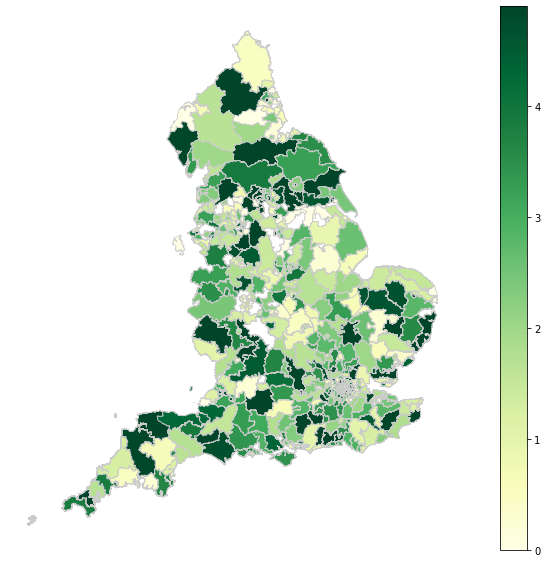
\includegraphics[width=0.55\textwidth]{overall_env_mentions_new.png}
	\caption{Mean Environmental Mentions By Constituency}
	\label{fig:meanenvbycon}
\end{wrapfigure}




The overall distribution of environmental mentions across England regardless of political party or election year is shown in Figure~\ref{fig:meanenvbycon}\footnote{Note: this figure only includes a narrower range of values, starting from the minimum value of 0 to the 90th percentile of the data in order to highlight more variation across constituencies. The overall map is shown in the appendix}. This groups the environmental mentions by constituency and then takes the mean for each of the constituencies. From this range of this figure, it is clear that there is very little variation across all constituencies regardless of year or party (with the exception of North Devon which appears to have an unusually high number of environmental mentions and is therefore not shown). It is unsurprising that there is little variation in this map as most of the variance is expected to be driven by political party and election year. 



In contrast, dividing the environmental mentions map by parties and election year shows considerably more variation. This is demonstrated in Figure~\ref{fig:parties_environmental_mentions} (Figures 4-8) for the 2010 Election with the Conservative, Green, Labour, Liberal Democrat, and UK Independence parties. Within these figures, it appears that the Conservative Party and Labour Party maps are relatively similar in variation, with similar constituencies showing up as most/least frequently mentioned. There appears to be slightly more variation in the Liberal Democrat map, with the Green Party and UK Independence Party maps appearing the most different. These results are interesting and unexpected as the Green Party seems to have relatively low numbers of mentions across all of England. This, however, may be caused because the Green Party is not considered to be one of the main parties in England, meaning that it is possible that there are simple less uploads of Green Party leaflets on the OpenElections website.







\begin{figure}[htbp]  % Use [htbp] for figure placement
	\centering
	
	% Row 1
	\begin{minipage}[t]{0.335\textwidth}
		\centering
		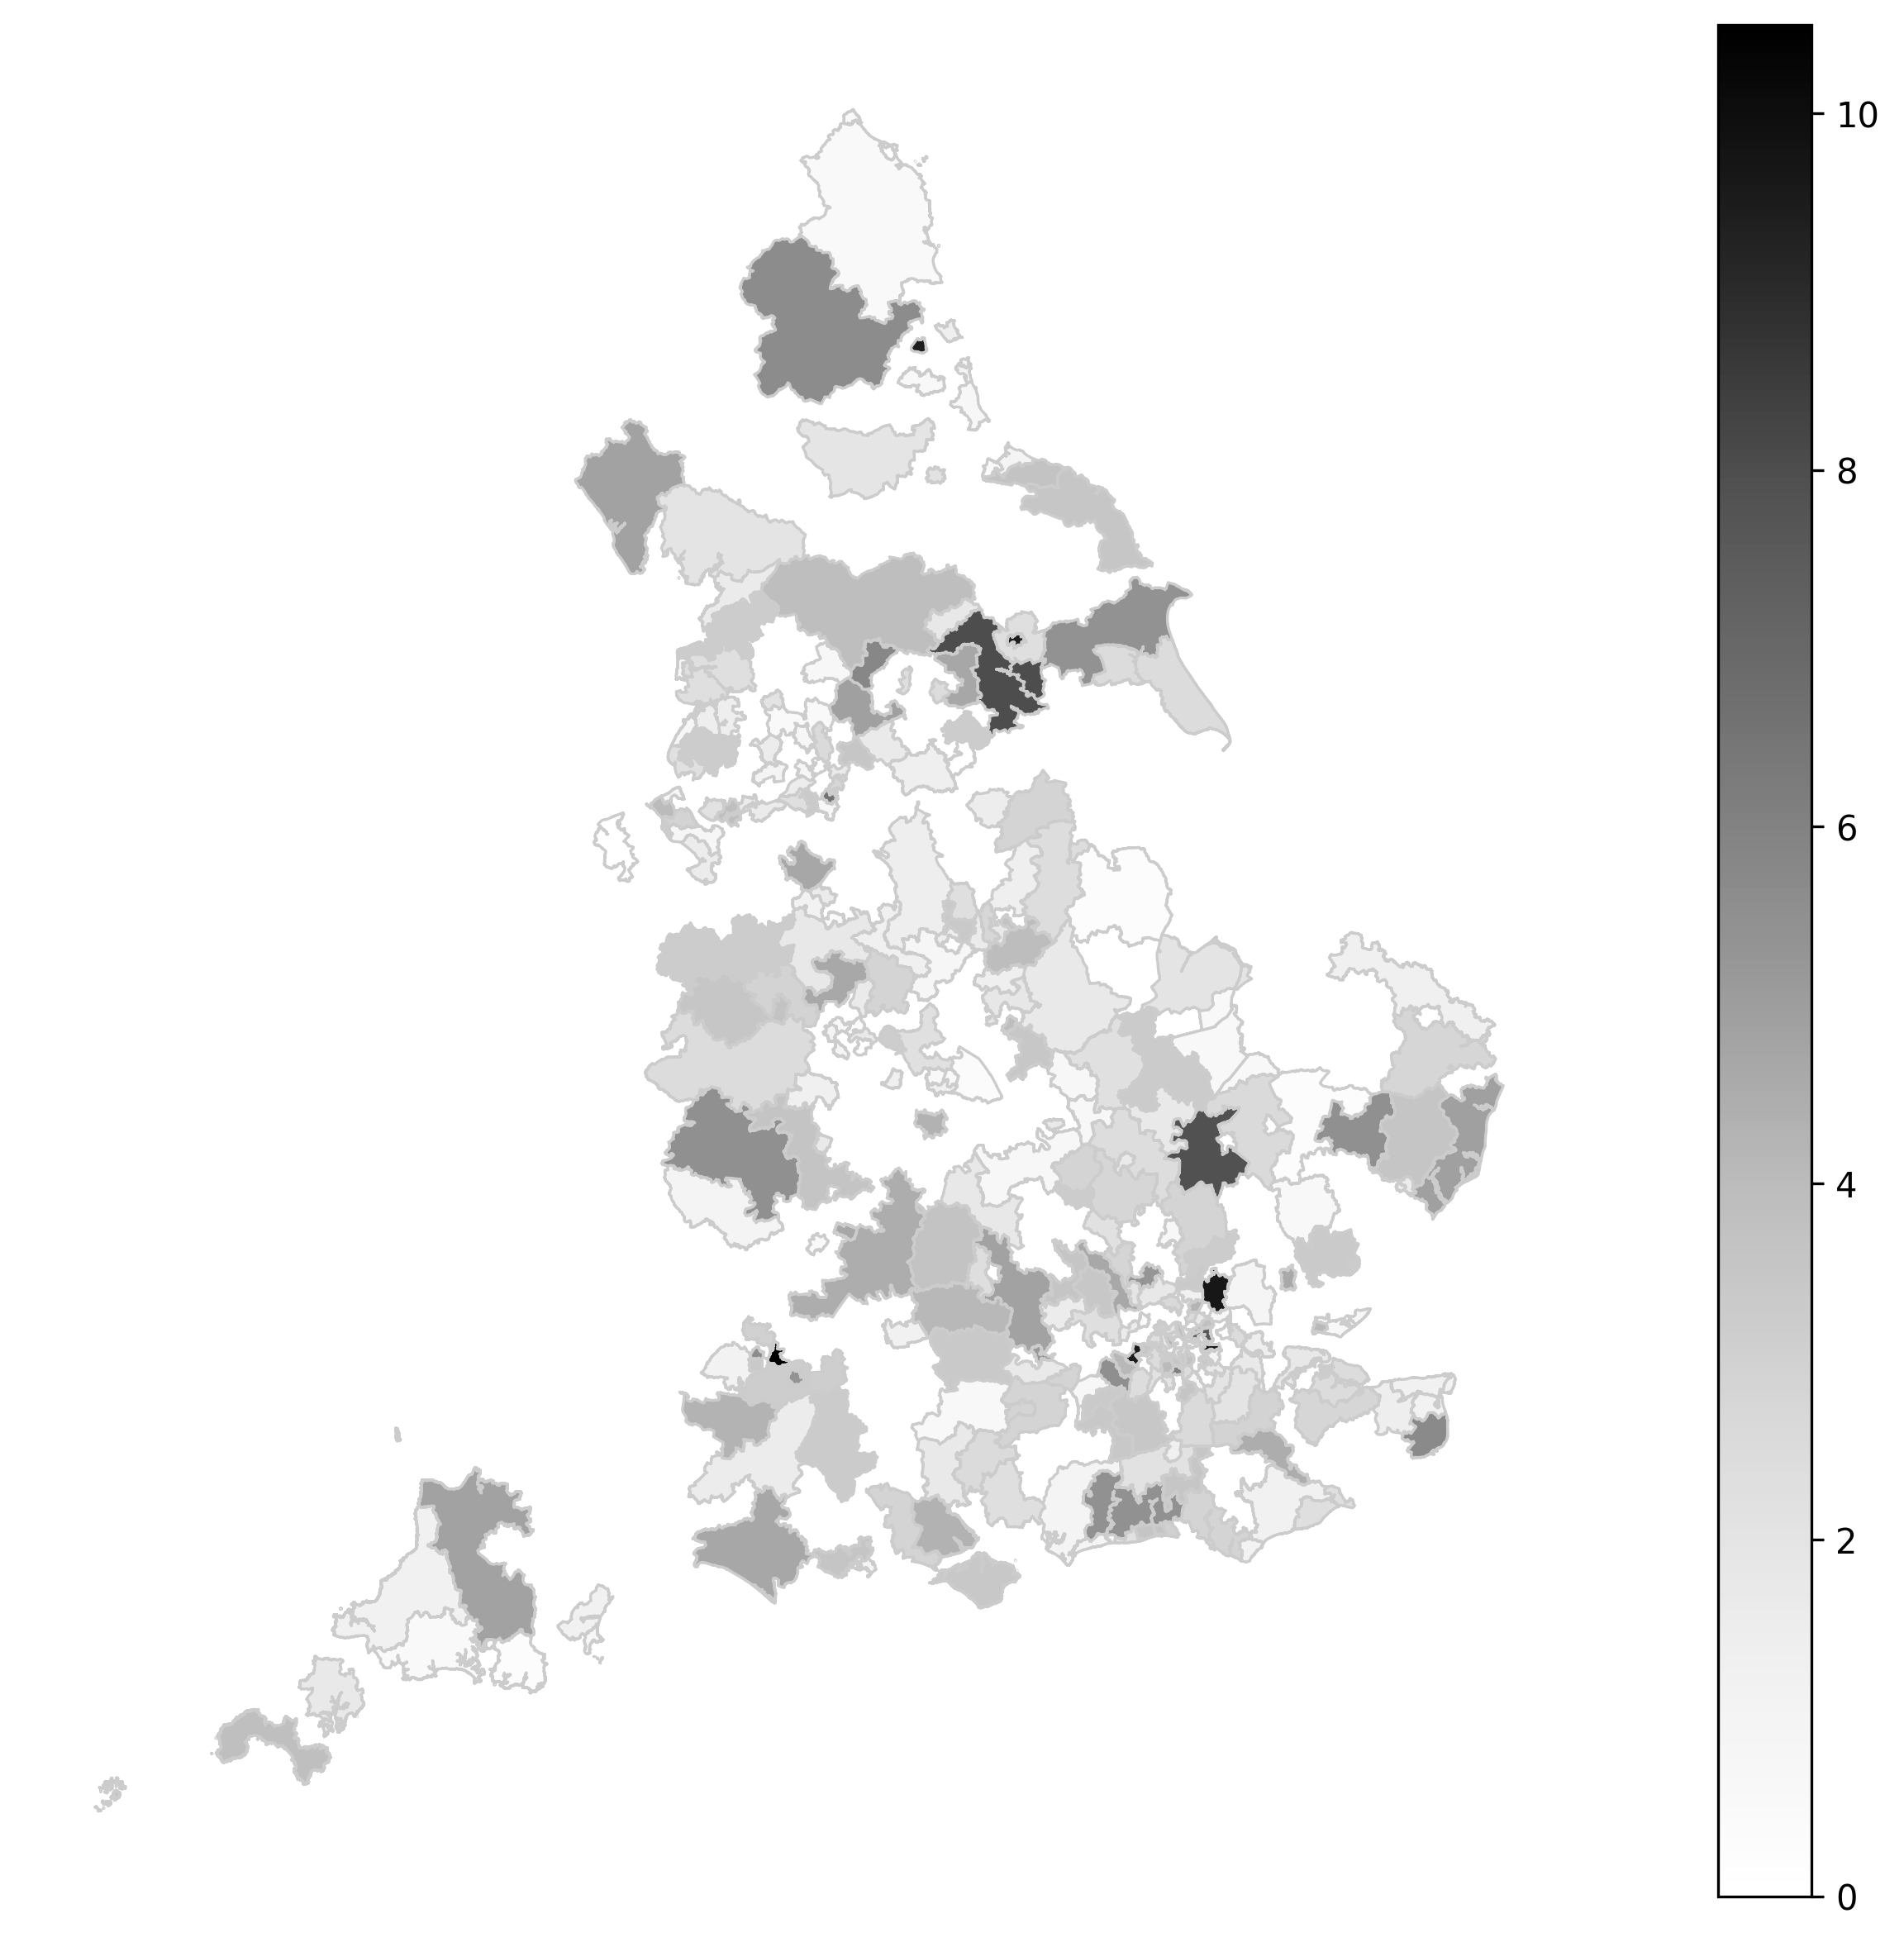
\includegraphics[width=\textwidth,height=0.68\textheight,keepaspectratio]{plots/ConservativeParty_2010GeneralElection_Environmental_Mentions.png}
		\caption{Conservative Party}
	\end{minipage}\hfill
	\begin{minipage}[t]{0.335\textwidth}
		\centering
		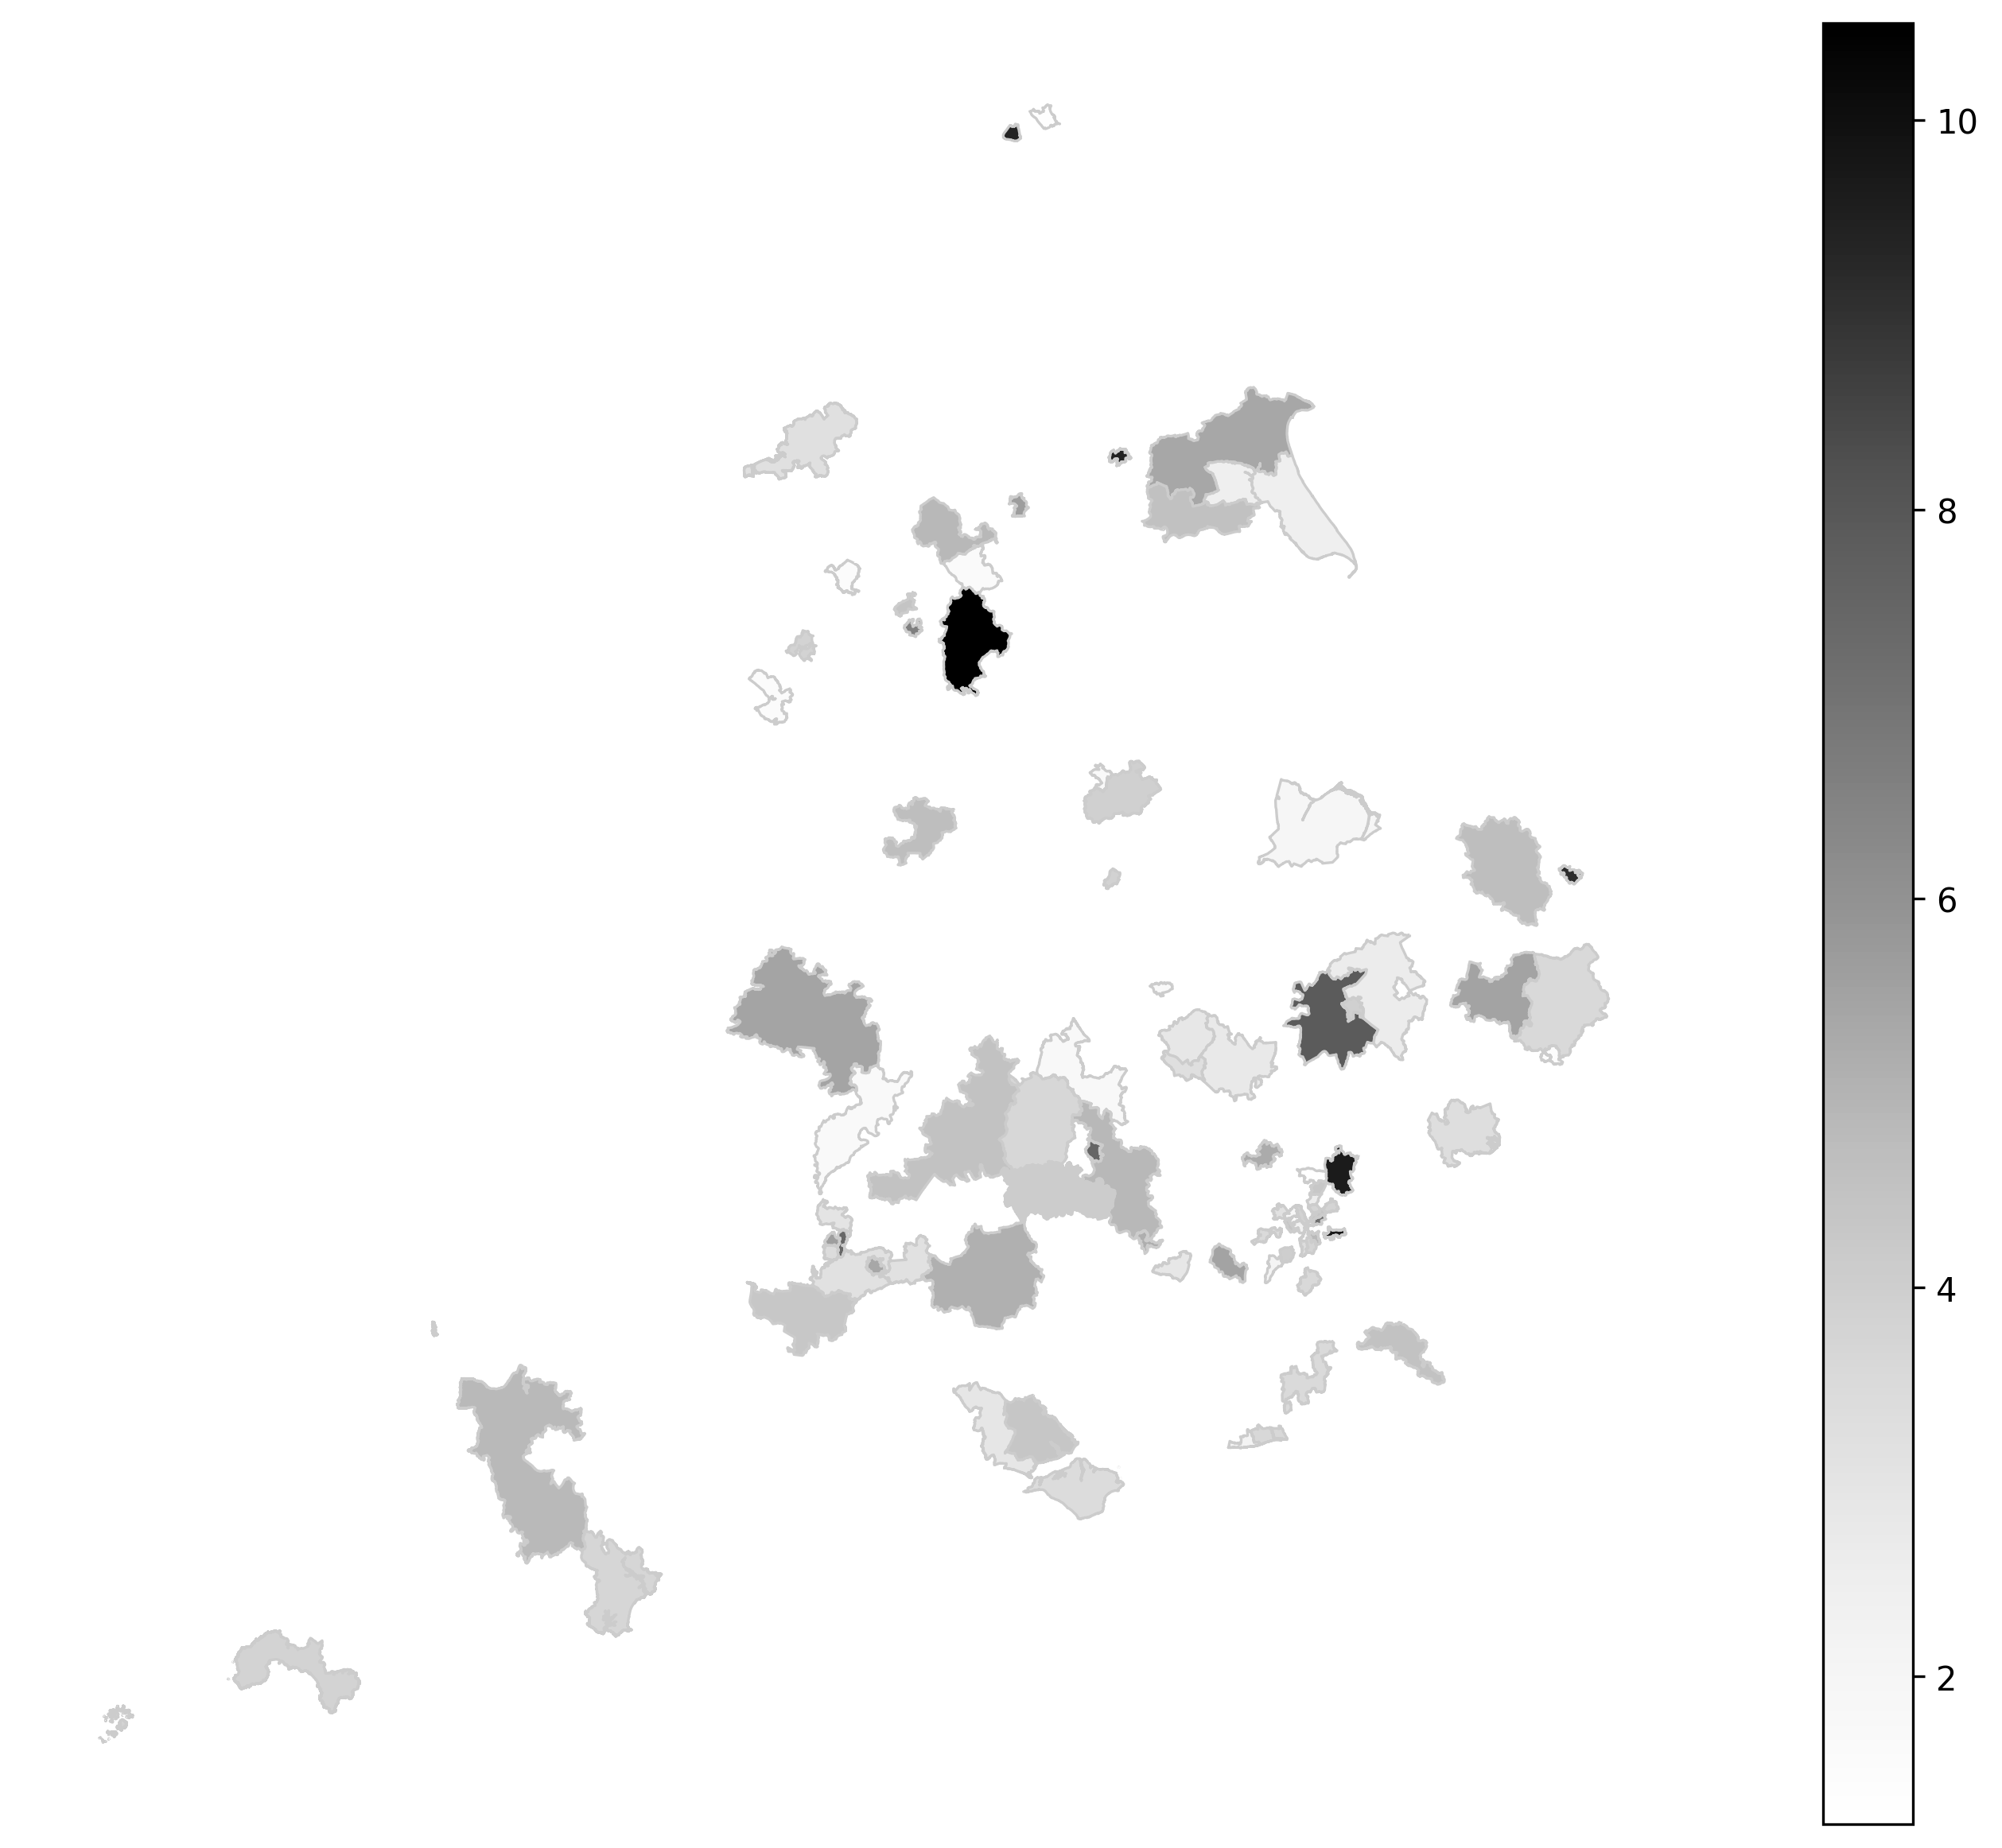
\includegraphics[width=\textwidth,height=0.68\textheight,keepaspectratio]{plots/GreenParty_2010GeneralElection_Environmental_Mentions.png}
		\caption{Green Party}
	\end{minipage}\hfill
	\begin{minipage}[t]{0.335\textwidth}
		\centering
		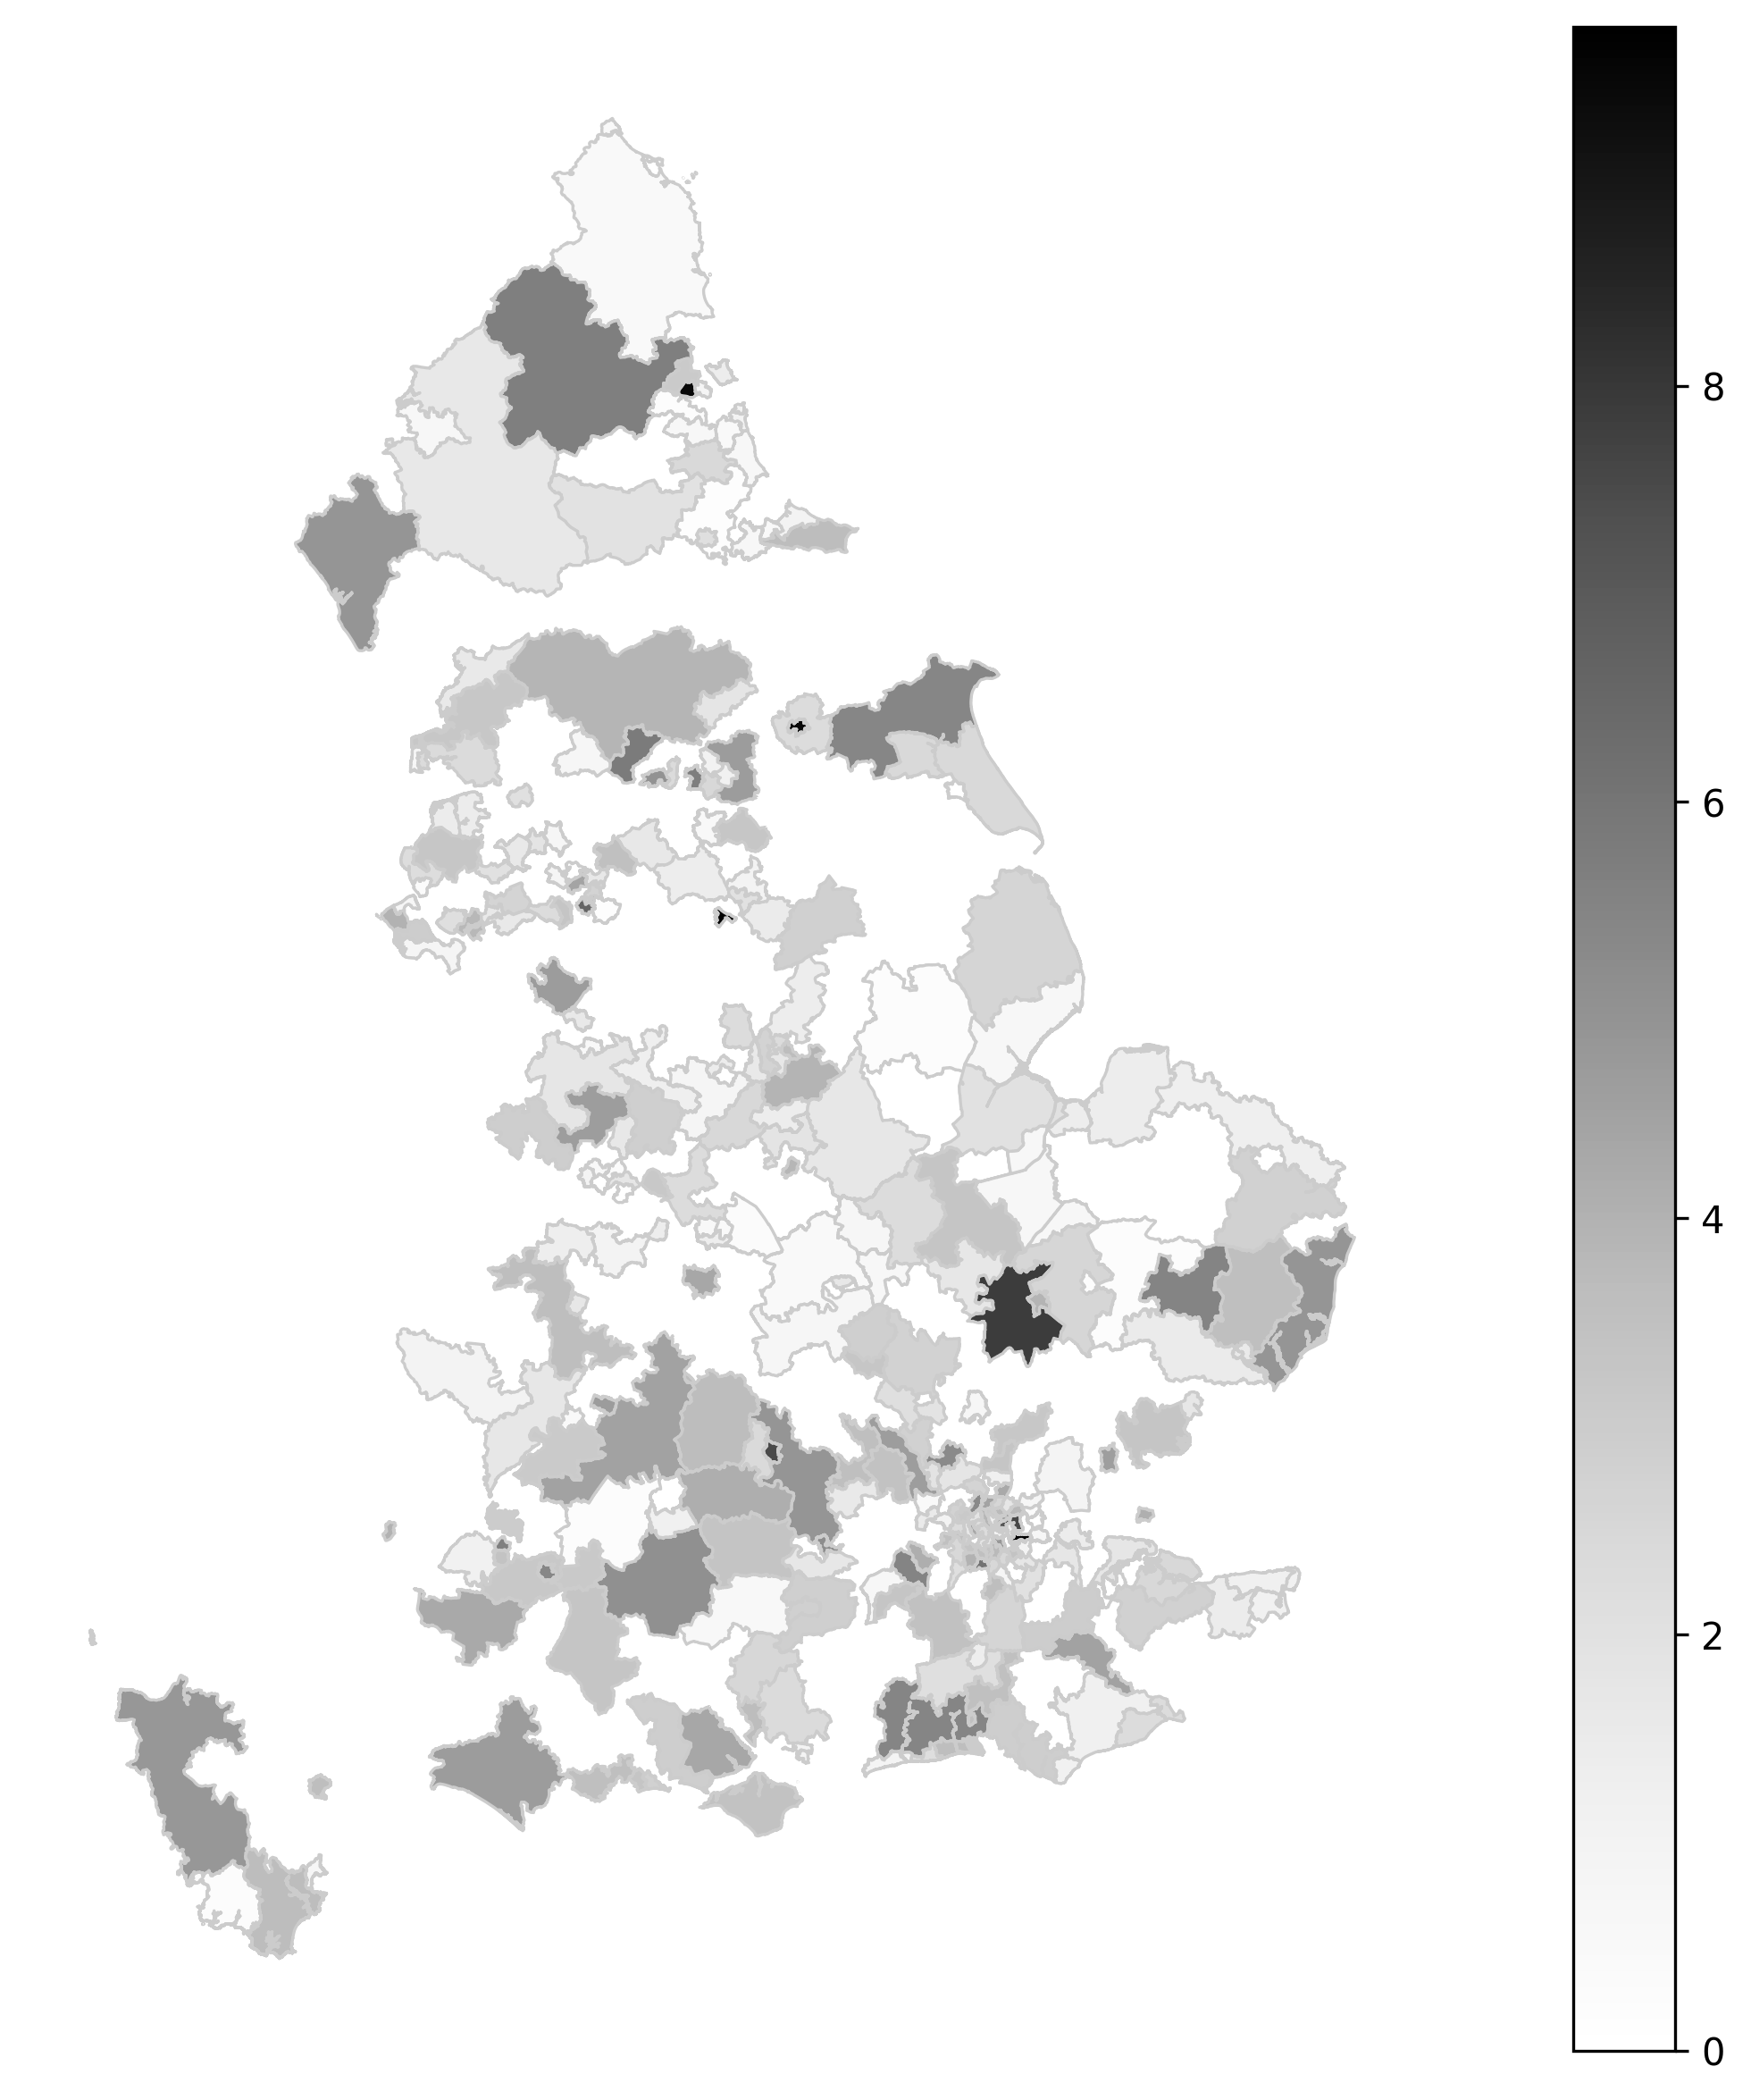
\includegraphics[width=\textwidth,height=0.68\textheight,keepaspectratio]{plots/LabourParty_2010GeneralElection_Environmental_Mentions.png}
		\caption{Labour Party}
	\end{minipage}
	
	\vspace{0.1cm}  % Adjust space between rows if necessary
	
	% Row 2
	\begin{minipage}[t]{0.335\textwidth}
		\centering
		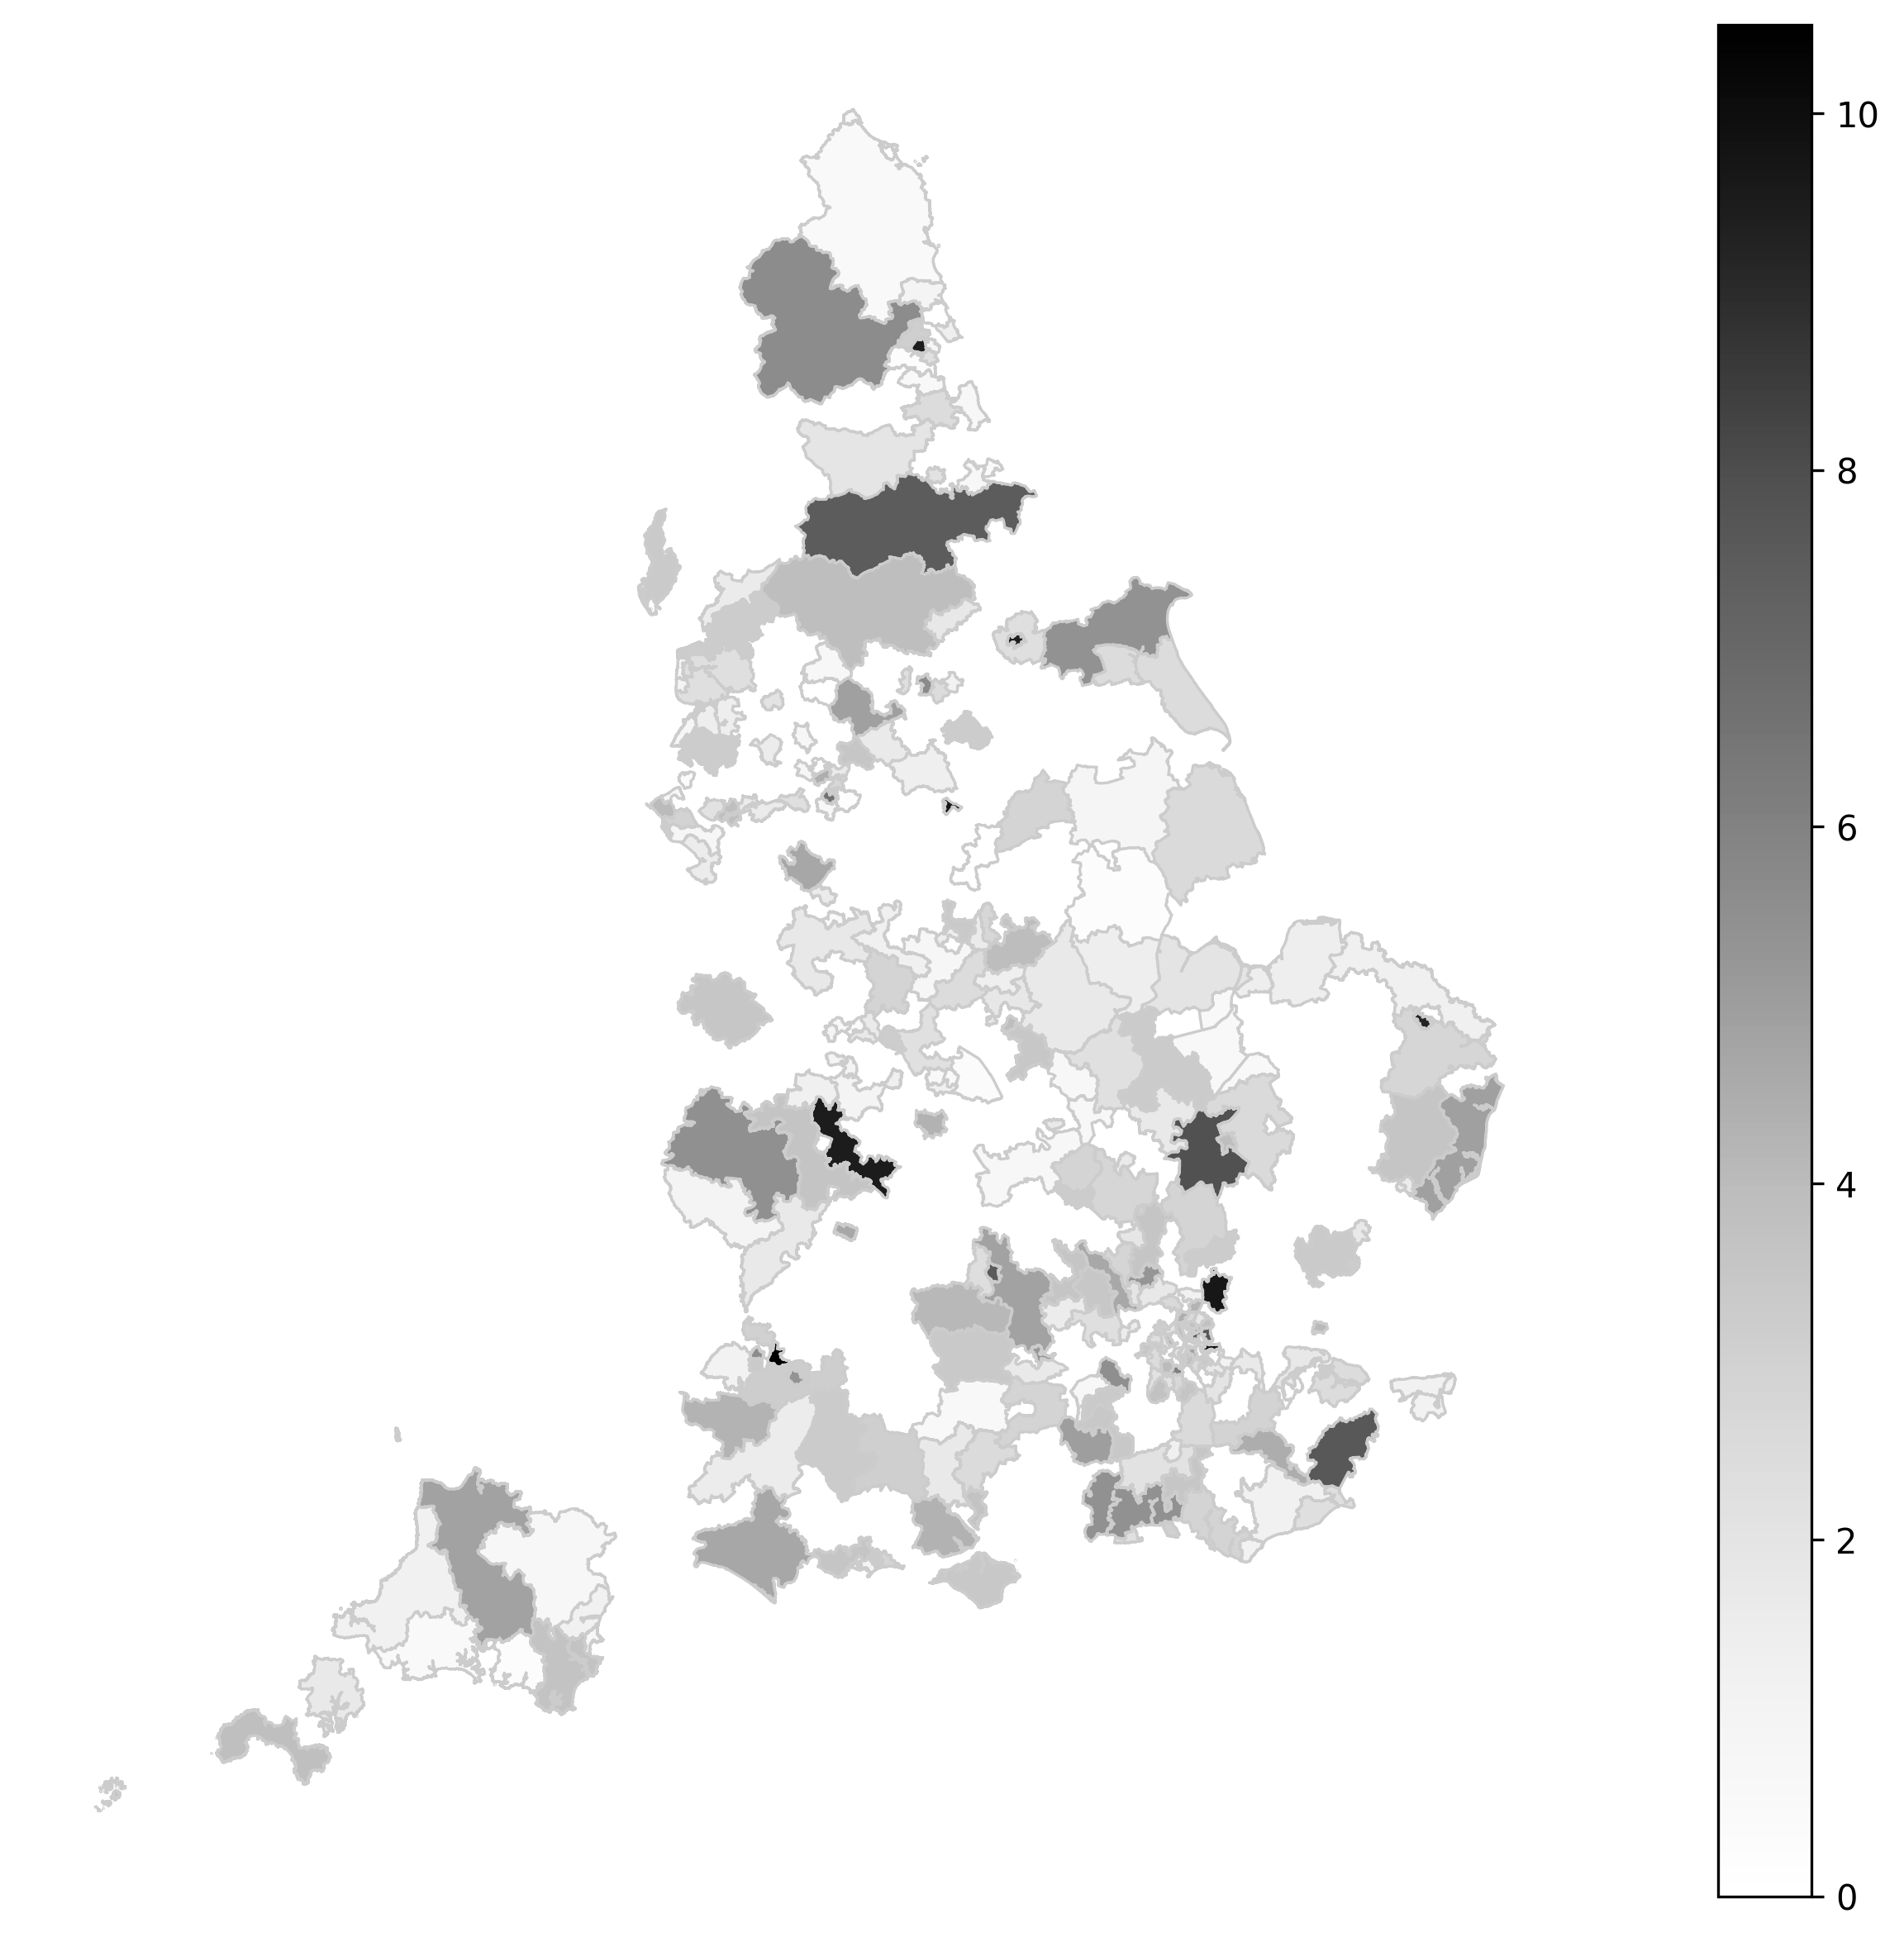
\includegraphics[width=\textwidth,height=0.68\textheight,keepaspectratio]{plots/LiberalDemocrats_2010GeneralElection_Environmental_Mentions.png}
		\caption{Liberal Democrats}
	\end{minipage}\hfill
	\begin{minipage}[t]{0.335\textwidth}
		\centering
		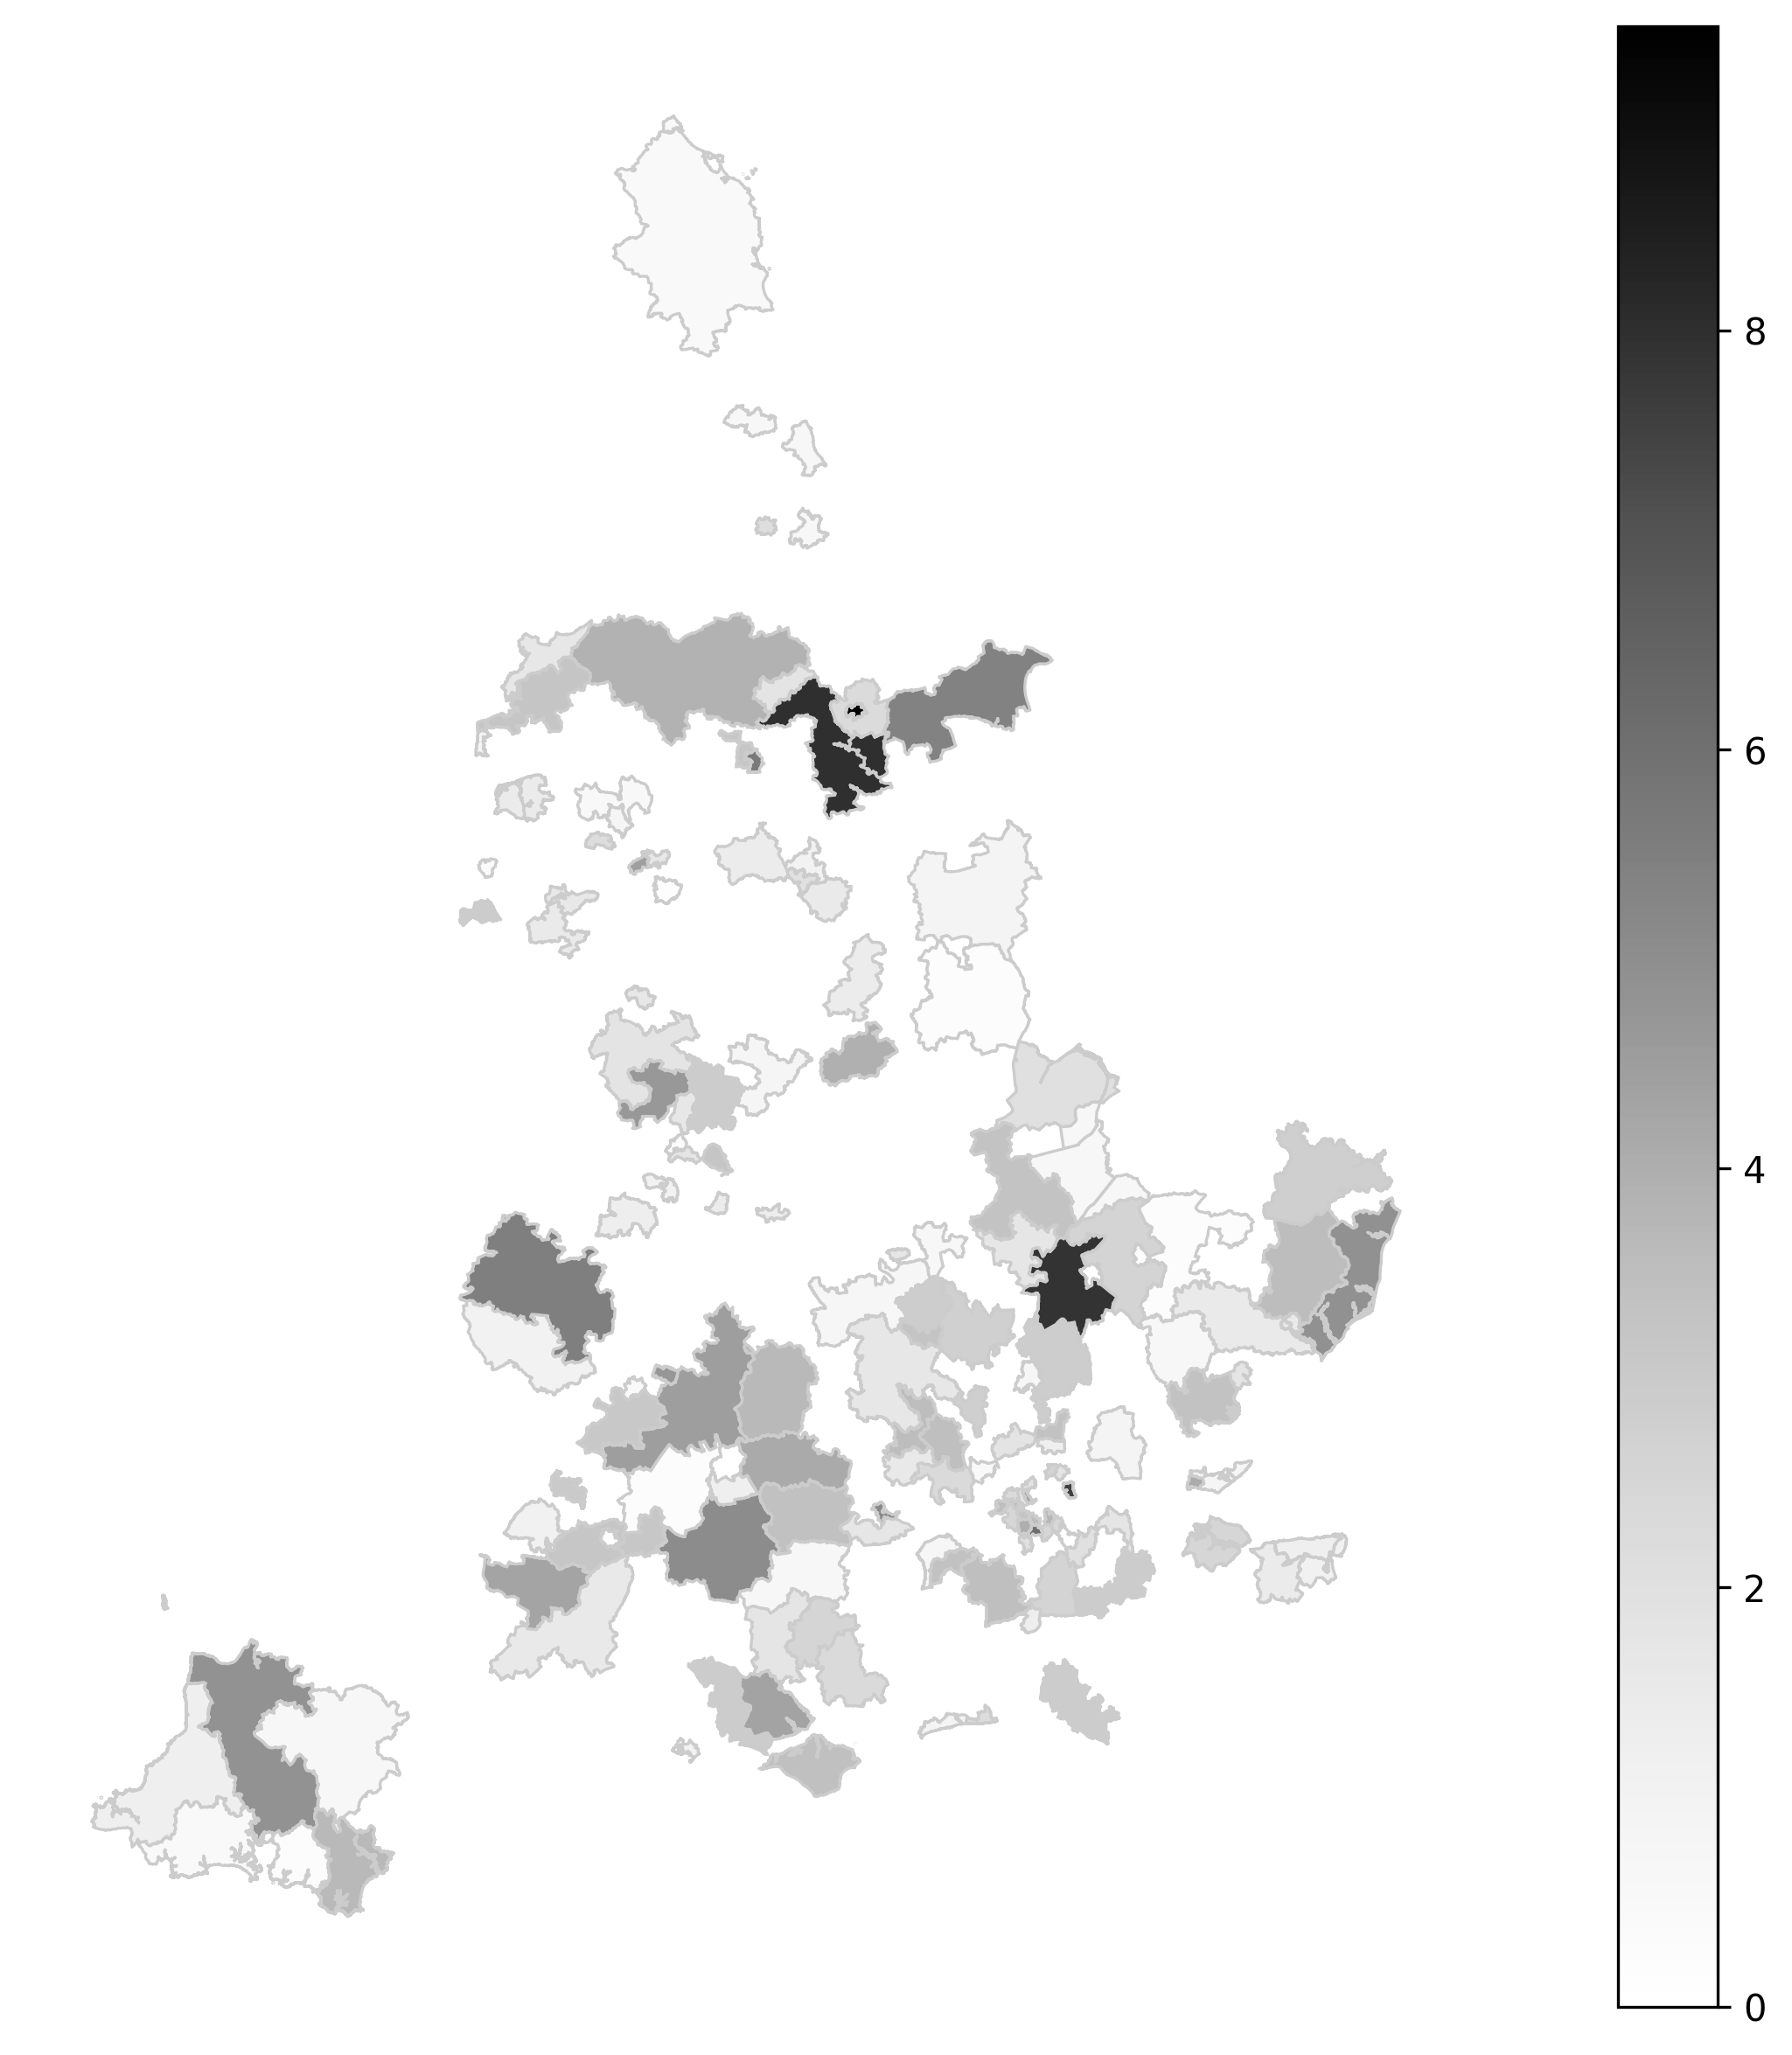
\includegraphics[width=\textwidth,height=0.68\textheight,keepaspectratio]{plots/UKIndependenceParty_2010GeneralElection_Environmental_Mentions.png}
		\caption{UK Independence Party}
	\end{minipage}
	
	\caption{Mean Environmental Mentions by Different Parties in the 2010 General Election}
	\label{fig:parties_environmental_mentions}
\end{figure}




As shown in Figure~\ref{fig:count_by_year}, the highest proportion of leaflets came from the 2015 and 2010 elections, with numbers significantly dropping in the 2017 and 2019 elections. This may be partially explained due to a shift to more online campaign styles, as social media campaigning may help politicians win more votes \citep{brightDoesCampaigningSocial2020}. Furthermore, the Green Party and the UK Independence Party have the lowest number of leaflets within the dataset, shown in Figure~\ref{fig:count_by_party_year}. The 2015 election contained the most number of leaflets for both of the aforementioned parties with the 2019 election showing the lowest number of leaflets for both parties. The Conservative, Labour, and Liberal Democrats contain more leaflets than the other two parties for each election year.  

The distribution of environmental mentions shown in Figure~\ref{fig:env_mentions_perc}, however, differs drastically from the overall distribution of leaflets by party and year. The Green Party, as to be expected, includes the highest percentage of environmental mentions for every election year included in the dataset. These mentions, aside from the 2015 election, continue to grow in percentage for each election year, such that environmental issues have been mentioned most in the 2017 and 2019 elections. All other included parties also show an increase in environmental mentions in the 2019 election, which may be caused by overall changes in environmental attitudes of the general public in recent years, as many voters have begun to see climate change as a primary topic in politics, leading politicians to be forced to incorporate these concerns in some way \citep{burnsWillBrexitDegrade2020}.



%descriptive stats








% Count of Observations by Year
\begin{figure}[htbp]  % Use [H] to place the figure exactly here
	\centering
	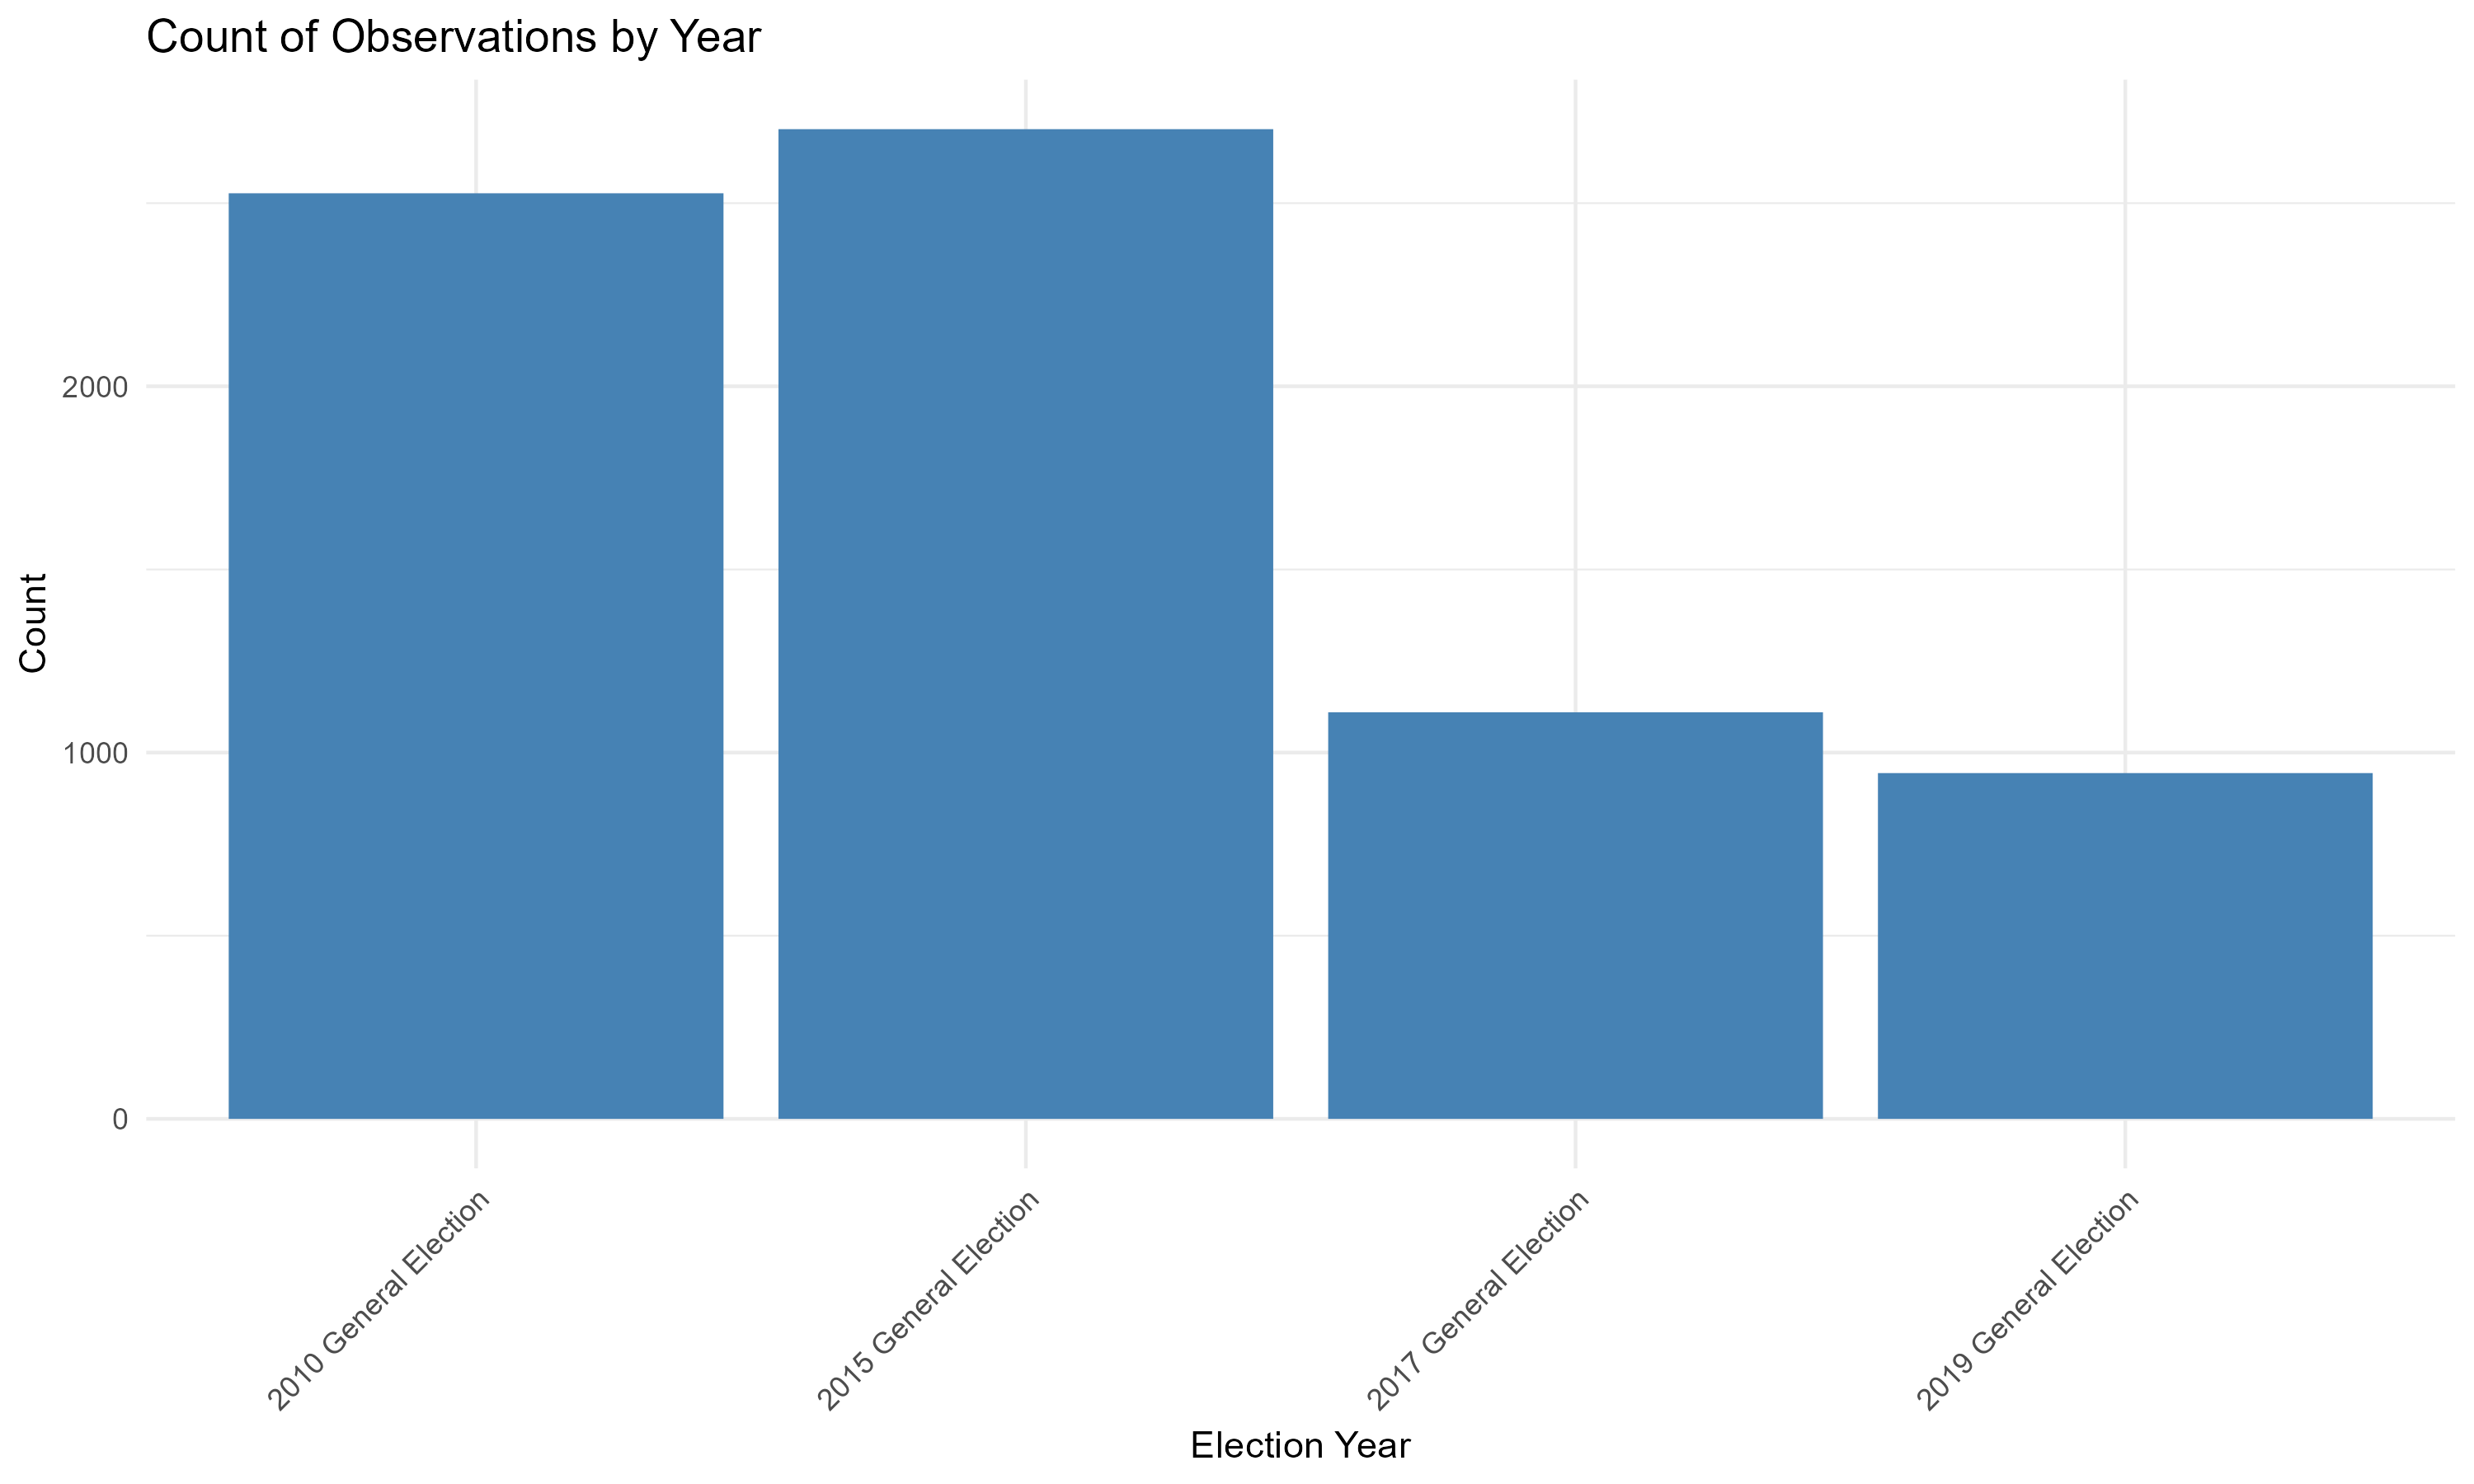
\includegraphics[width=\textwidth, height=0.7\textheight, keepaspectratio]{count_by_year.png} % Use full text width, adjust height
	\caption{Count of Observations by Year}
	\label{fig:count_by_year}
\end{figure}




% Count of Observations by Party and Year
\begin{figure}[htbp]
	\centering
	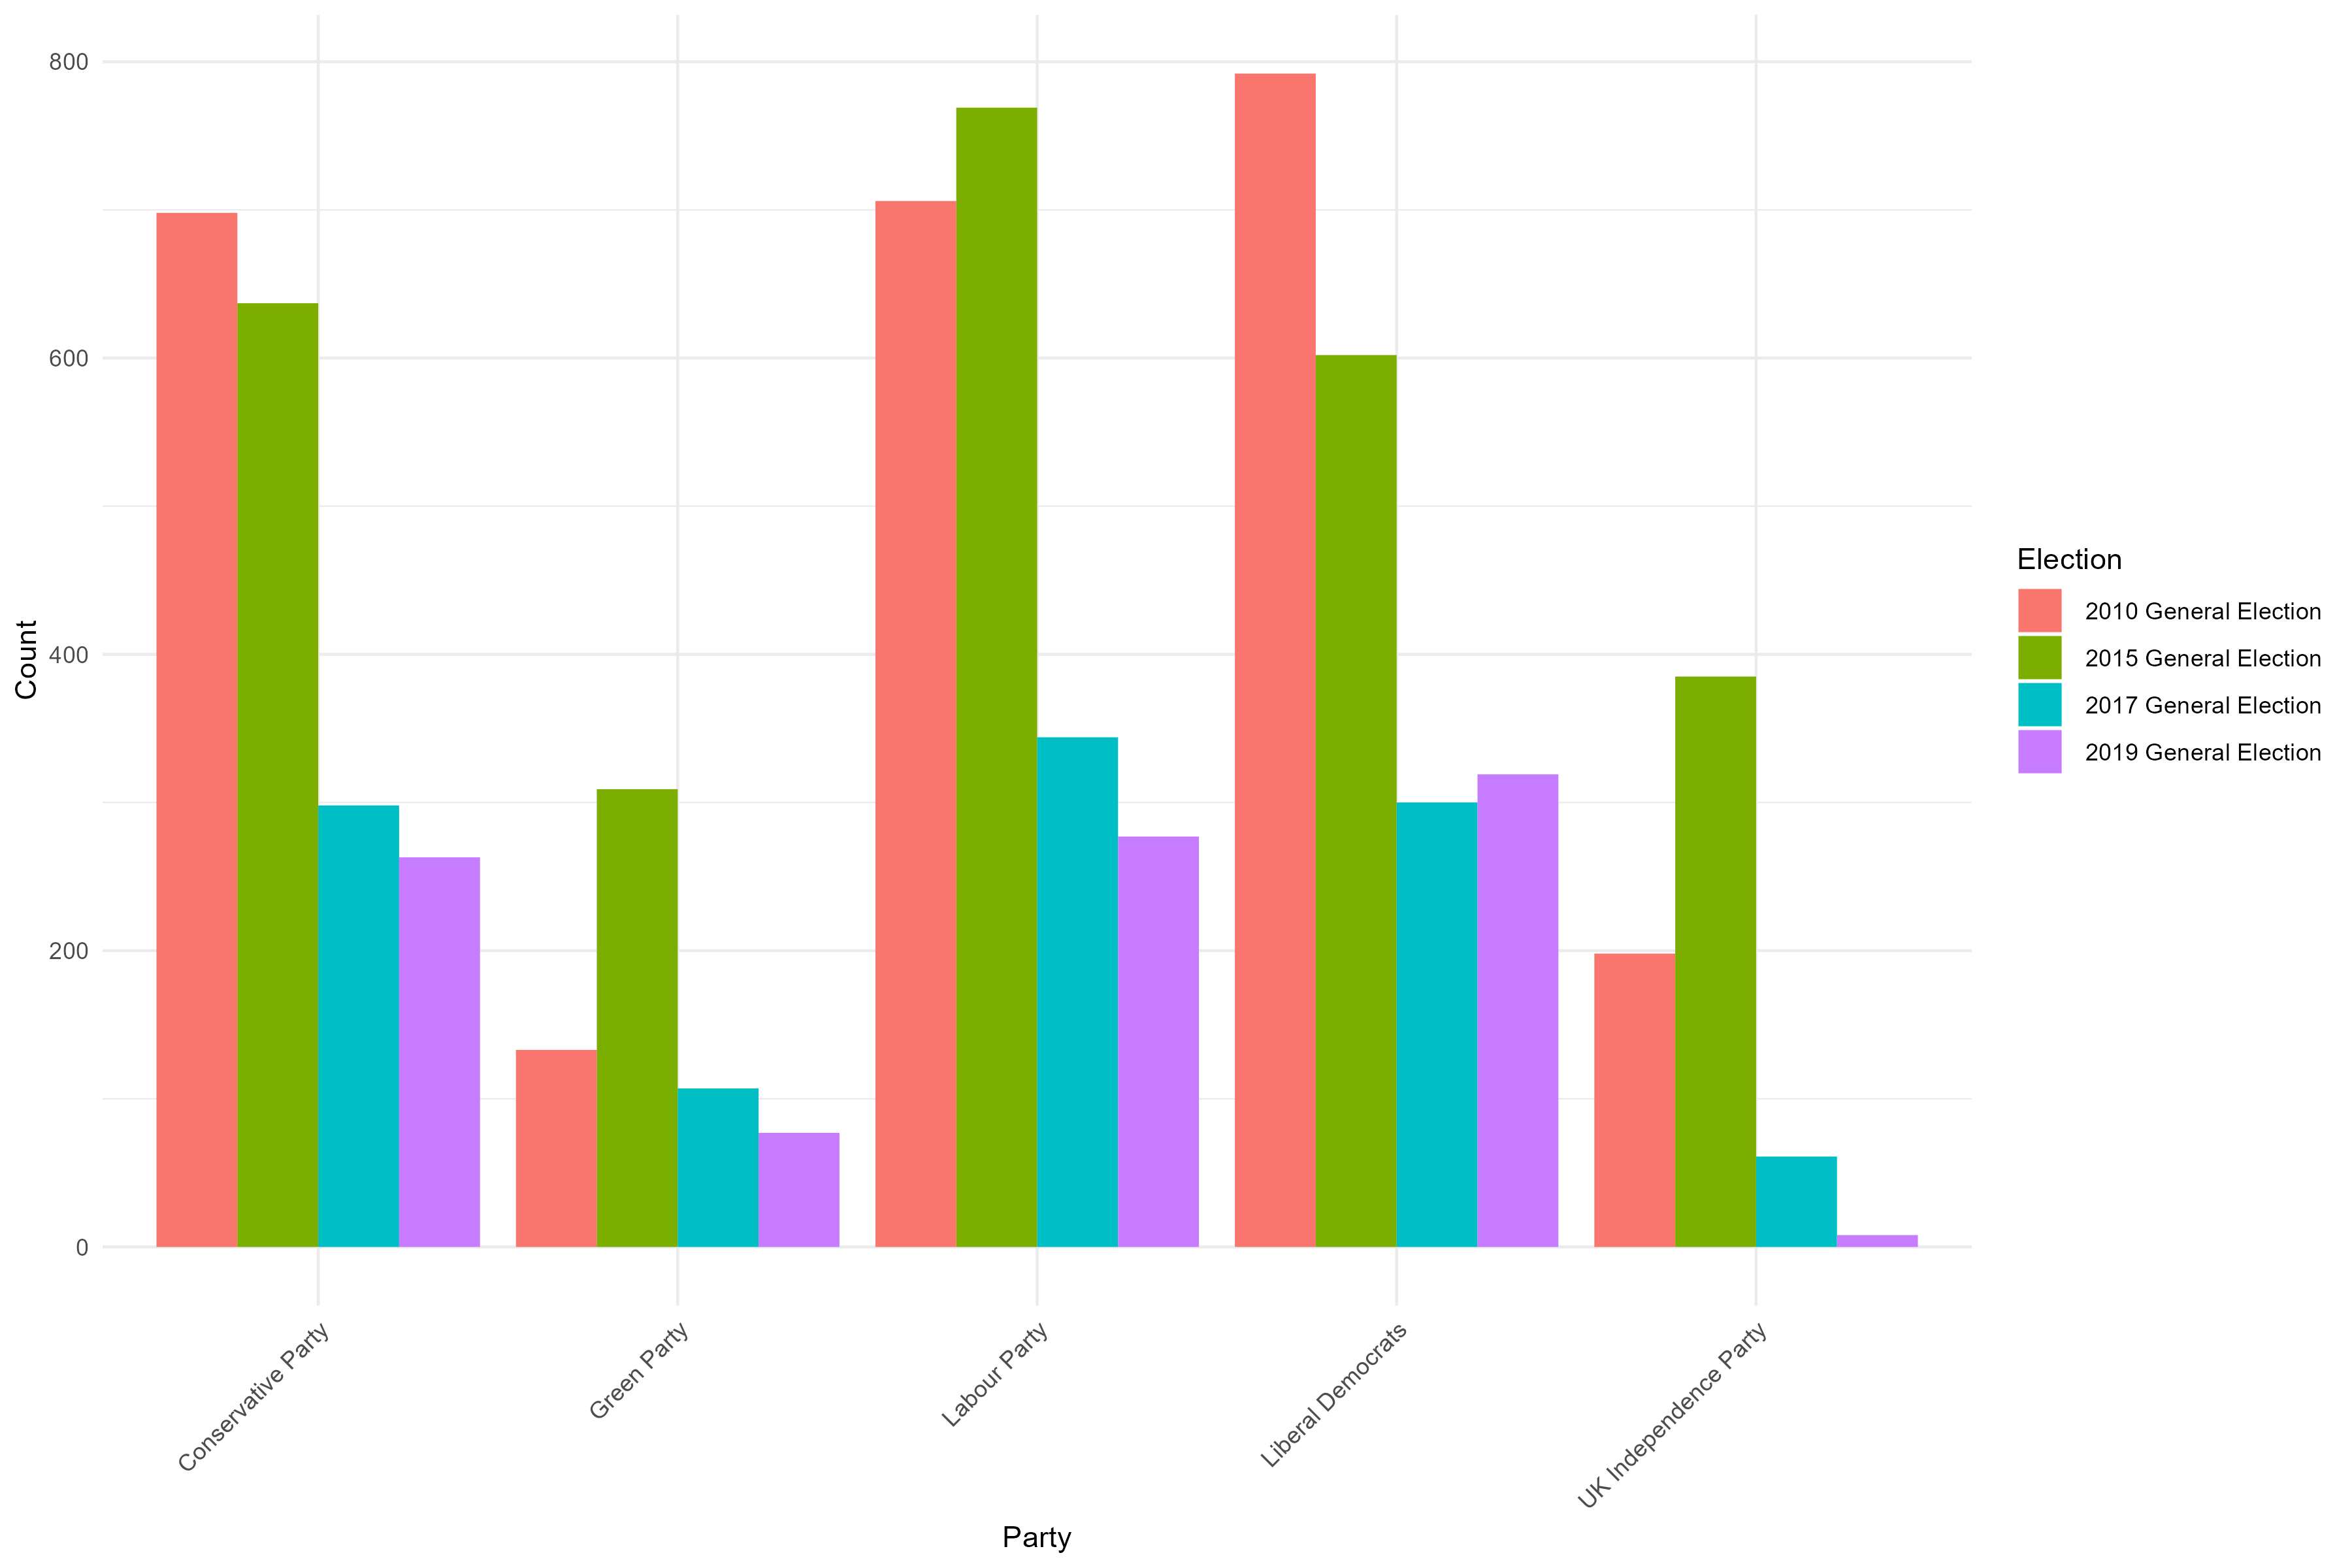
\includegraphics[width=\textwidth, height=0.6\textheight, keepaspectratio]{count_by_party_year.png} % Use full text width, adjust height
	\caption{Count of Observations by Party and Year}
	\label{fig:count_by_party_year}
\end{figure}

\vspace{-1cm}
% Percentages
\begin{figure}[htbp]
	\centering
	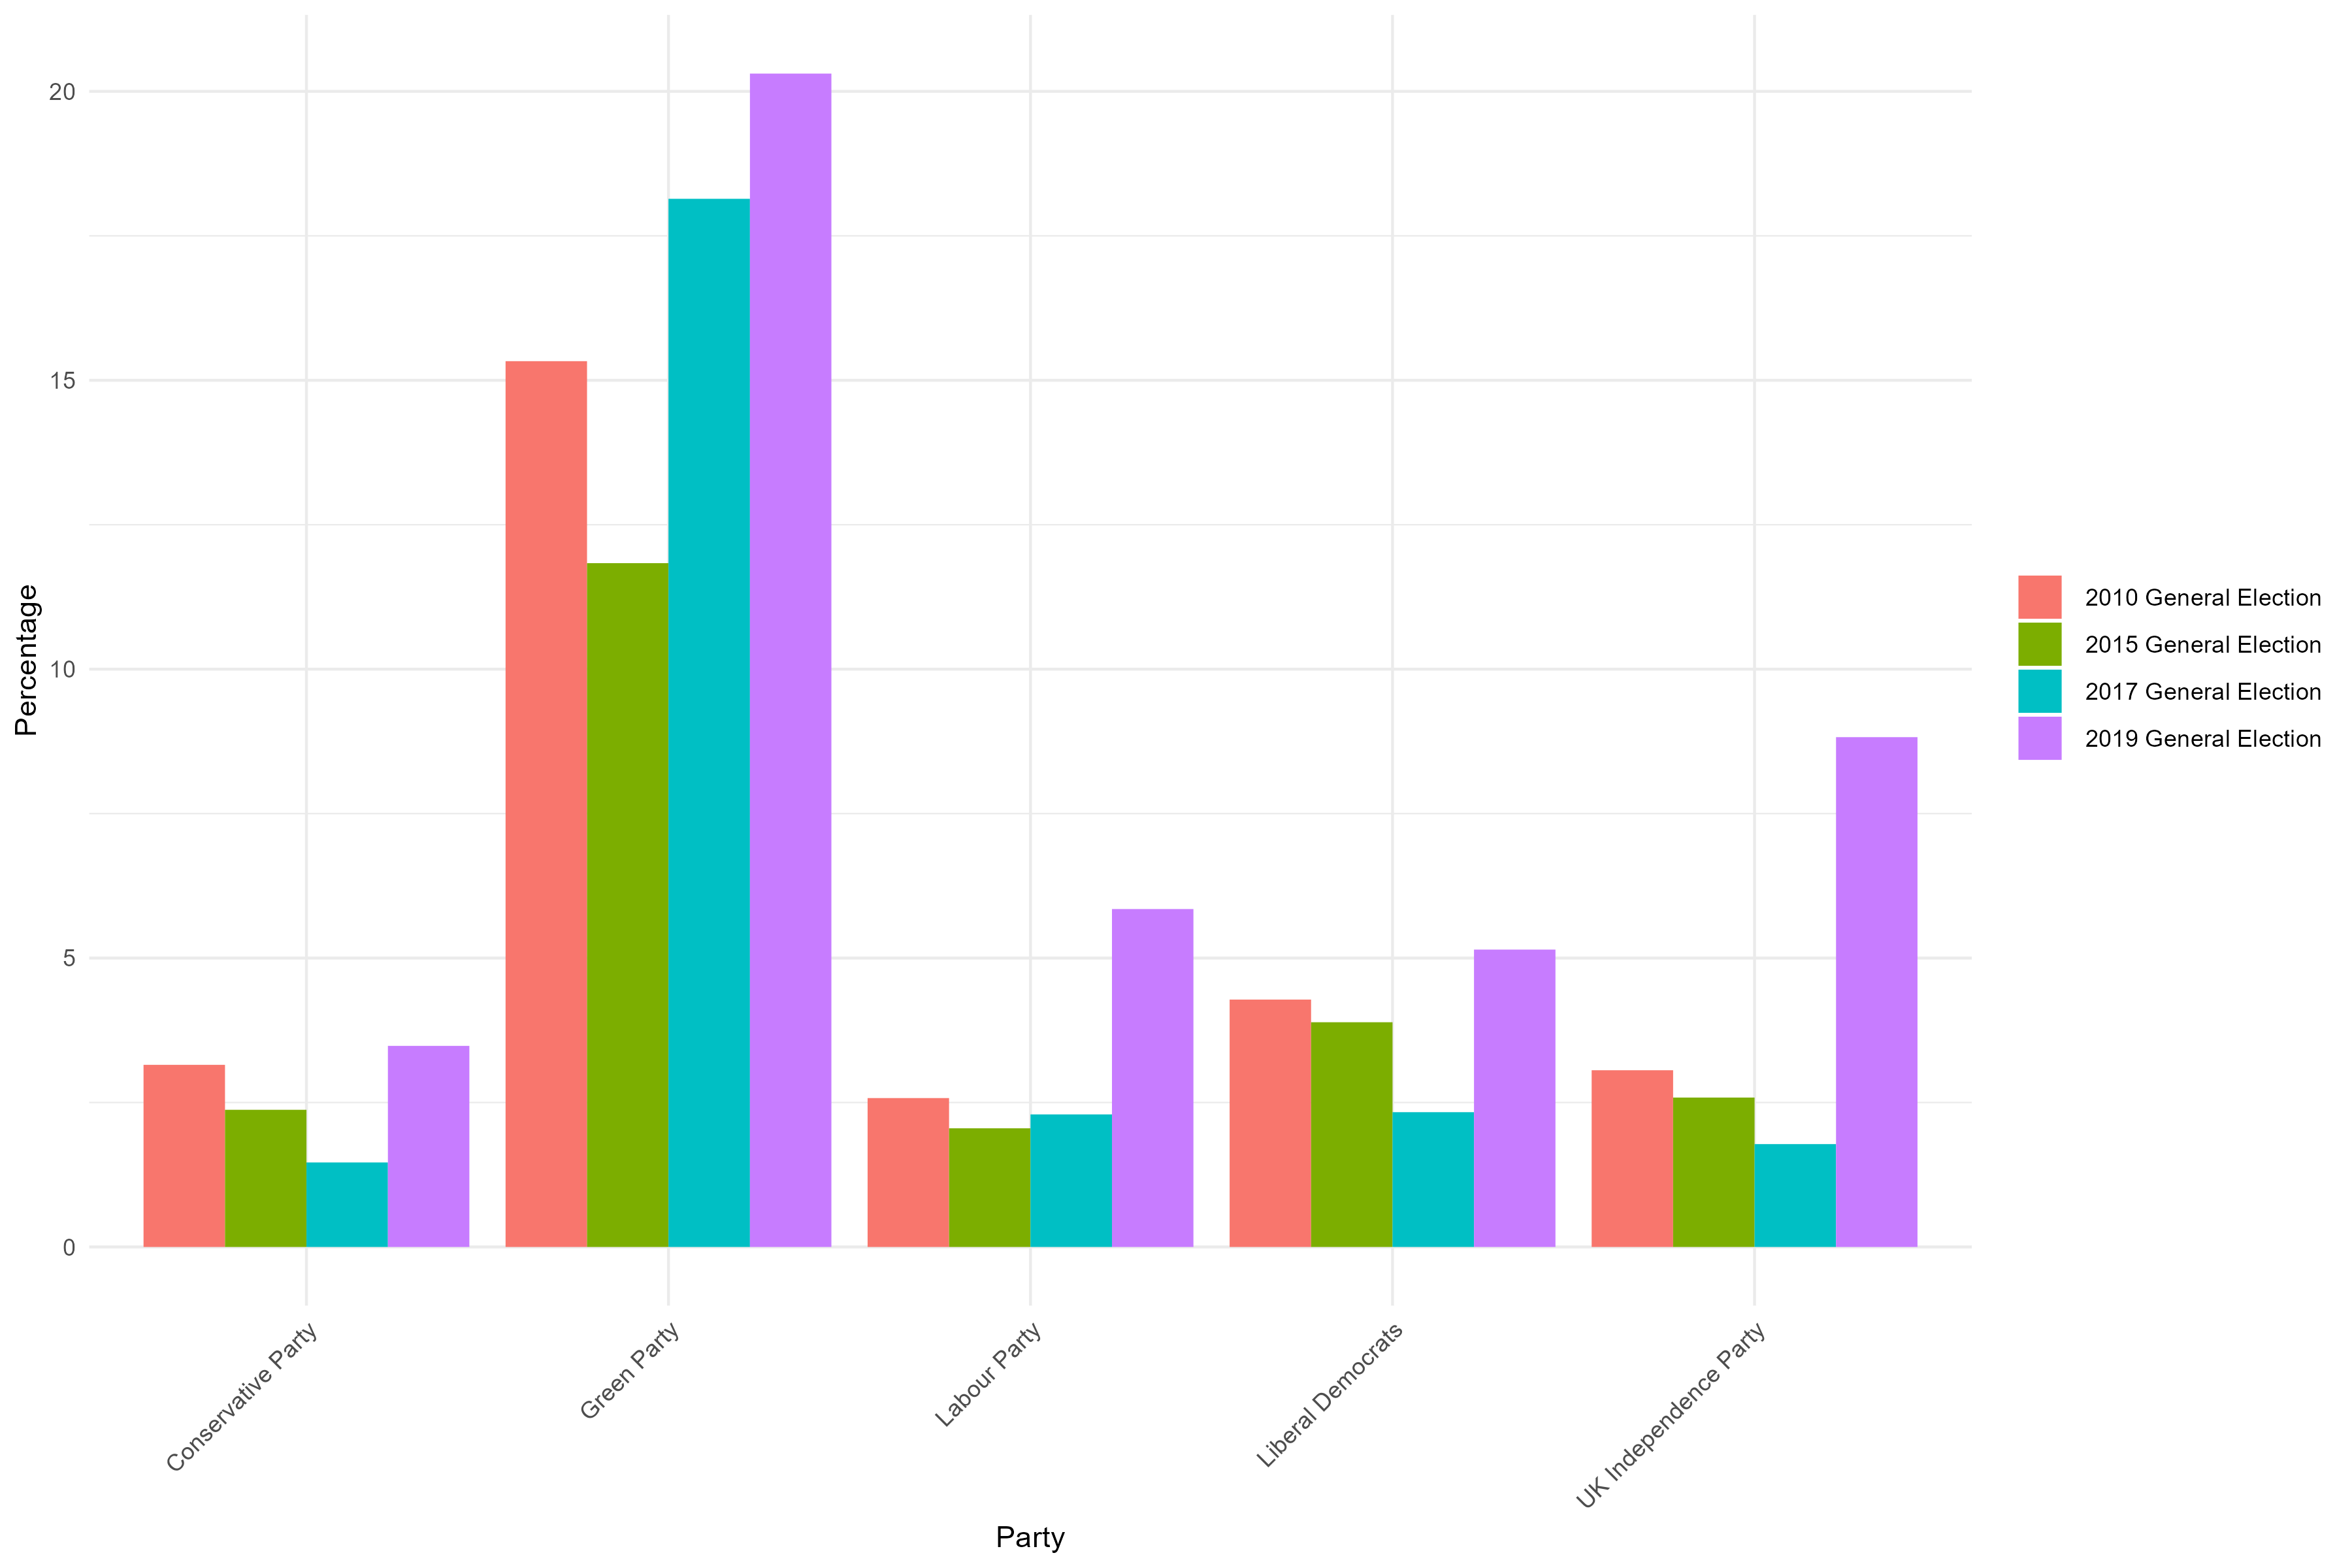
\includegraphics[width=\textwidth, height=0.6\textheight, keepaspectratio]{env_mentions_percentage.png} % Use full text width, adjust height
	\caption{Percentage of Environmental Mentions by Party and Year}
	\label{fig:env_mentions_perc}
\end{figure}


\newpage

As the descriptive statistics indicate significant variation in environmental mentions by year and party, 9 multivariate linear regression analyses were conducted. The first, shown in Table 3, includes both election year and political party as dummy variables in the predictors. Table 4 shows the next four models which include political party as dummy variables, with each regression referring to each election year. Table 5 shows regression results for each of the political parties.



\subsection{Two-Way Fixed Effect Model Results}

Table~\ref{tab:2wfe} presents the results of the two-way fixed effects model, which controls for both political party effects and constituency-specific effects in addition to election-year fixed effects. By including both constituency and time fixed effects, this model allows us to account for unobserved heterogeneity at the constituency level and observe how environmental mentions vary both over time (across elections) and across constituencies.

The inclusion of constituency fixed effects is particularly important because for control over factors that may differ across constituencies, removing the need for inclusion of many covariates, instead isolating the focus to political party alone. This therefore explains whether the variance that is seen in the previous models is due to political party and year alone.

The non-significant results across all political parties suggest that, after controlling for constituency-specific factors, there is no significant variation in the presence of environmental mentions across political party. This implies that it may be more important to look specifically at what causes variation within each constituency, rather than assuming the political party is the driving force in the variation shown.


\subsection{One-Way Fixed Effect Model Results}

Table~\ref{tab:1wfe} shows the results of a one-way fixed effects model that includes political party controls and election-year fixed effects. The model controls for variation across different election years, allowing for observation of which factors within constituencies had the strongest effect on environmental mention count, account for variance specific to election-year effects. This is the first step in isolating which factors specifically are responsible for the mechanism of environmental mentions by insuring that the model is not picking up variance that can be explained by the election year alone.

For the Conservative Party, the fixed effect coefficient is \(-1.34\) \((p < 0.01)\). This suggests that, on average, environmental mentions in the Conservative Party's campaigns were lower by 1.34 points, relative to the overall election-year trend.

Similarly, the Labour Party has a coefficient of \(-1.384\) \((p < 0.01)\), indicating a decrease of 1.384 points in environmental mentions compared to the baseline election year (2010). The Liberal Democrats show a slightly smaller decrease at \(-1.317\) points \((p < 0.01)\). Lastly, the UK Independence Party shows the largest decrease with a coefficient of \(-1.574\) \((p < 0.01)\).

Controlling for variance across elections that is not included through covariates in the model demonstrates that the political party defining the campaign messages has a significant effect in how often environmental issues are presented to constituents. 

Outside of political party, the other variables that were shown to be significant in explaining variance of environmental mentions were certain occupations, students, and weather. Overall student count is associated with an increase in environmental mentions in a constituency $(p < 0.01)$. An effect in the same direction is observed with overall weather variation, with a 1 point increase in weather variance associated with a 0.044 point increase in environmental mentions $(p < 0.01)$. An inverse effect is observed with the count of routine workers, with an increase in routine workers associated with a decrease in environmental mentions.




% Table 1: Fixed Effects Model with Election-Year Controls (Time and Constituency)
\begin{table}[htbp]  % Use [htbp] instead of [H]
	\centering
	\caption{Fixed Effects Model with Election-Year Controls (Time and Constituency)}
	\label{tab:2wfe}
	\setlength{\tabcolsep}{10pt} % Adjust column spacing for better presentation
	\begin{tabular}{@{\extracolsep{5pt}}lc}
		\hline
		& \multicolumn{1}{c}{\textit{Dependent variable:}} \\
		\cline{2-2}
		& Mean Environmental Mentions \\
		\hline
		Conservative Party & 0.000 \\
		& (0.000) \\
		Labour Party & 0.000 \\
		& (0.000) \\
		Liberal Democrats & $-$0.000 \\
		& (0.000) \\
		UK Independence Party & 0.000 \\
		& (0.000) \\
		\hline
		Observations & 3,106 \\
		R$^{2}$ & 0.096 \\
		Adjusted R$^{2}$ & $-$0.070 \\
		\hline
		\multicolumn{2}{l}{\footnotesize{Note: $^{*}$p$<$0.1; $^{**}$p$<$0.05; $^{***}$p$<$0.01}} \\
	\end{tabular}
\end{table}

\vspace{0.5cm}  % Adjust spacing between tables

% Table 2: Fixed Effects Model with Election-Year Controls
\begin{table}[htbp]  % Use [htbp] instead of [H]
	\centering
	\caption{Fixed Effects Model with Election-Year Controls}
	\label{tab:1wfe}
	\footnotesize
	\setlength{\tabcolsep}{8pt} % Adjust column spacing for better presentation
	\begin{tabular}{lcc}
		\toprule
		\textbf{Variable} & \textbf{Coef.} & \textbf{SE} \\
		\midrule
		\textit{Party Dummies} \\
		\hspace{3mm}Conservative Party & $-1.343^{***}$ & (0.202) \\
		\hspace{3mm}Labour Party & $-1.384^{***}$ & (0.200) \\
		\hspace{3mm}Liberal Democrats & $-1.317^{***}$ & (0.203) \\
		\hspace{3mm}UKIP & $-1.574^{***}$ & (0.232) \\
		\textit{Demographics} \\
		\hspace{3mm}Median Age & $-0.006$ & (0.032) \\
		\hspace{3mm}Students Count & $0.0001^{***}$ & (0.00004) \\
		\textit{Population} \\
		\hspace{3mm}Rural Pop. & $-0.00000$ & (0.00003) \\
		\hspace{3mm}Urban Pop. & $-0.00002$ & (0.00003) \\
		\textit{Occupation Shares} \\
		\hspace{3mm}Higher Managerial & $-0.00001$ & (0.0001) \\
		\hspace{3mm}Lower Managerial & $0.0001$ & (0.0001) \\
		\hspace{3mm}Intermediate & $0.00004$ & (0.0001) \\
		\hspace{3mm}Small Employers & $0.0001$ & (0.0001) \\
		\hspace{3mm}Lower Supervisory & $0.0002$ & (0.0002) \\
		\hspace{3mm}Semi Routine & $0.00001$ & (0.0001) \\
		\hspace{3mm}Routine & $-0.0002^{**}$ & (0.0001) \\
		\hspace{3mm}Never Worked & $-0.0001$ & (0.0001) \\
		\hspace{3mm}Long-term Unemp. & $0.0003$ & (0.0003) \\
		\textit{Other Controls} \\
		\hspace{3mm}Weather Variation & $0.044^{***}$ & (0.014) \\
		\textit{Party Shares} \\
		\hspace{3mm}Lib Dem Share & $-0.137$ & (0.993) \\
		\hspace{3mm}Labour Share & $-0.131$ & (0.992) \\
		\hspace{3mm}Other Share & $-0.131$ & (0.993) \\
		\hspace{3mm}Conservative Share & $-0.142$ & (0.993) \\
		\midrule
		Observations & \multicolumn{2}{c}{2,231} \\
		R$^2$ / Adj. R$^2$ & \multicolumn{2}{c}{0.157 / -0.620} \\
		\bottomrule
		\multicolumn{3}{l}{\footnotesize{$^{*}$p$<$0.1; $^{**}$p$<$0.05; $^{***}$p$<$0.01}} \\
	\end{tabular}
\end{table}



\newpage



\section{Discussion}


The time period analysed in this project provides an interesting and complicated political atmosphere to navigate. Given the Brexit referendum in 2016, there was a shift towards two-party politics in England in the 2017 election \citep{hoboltBrexit2017UK2018,prosserStrangeDeathMultiparty2018}, as voters who may have previously voted for the UK Independence shifted loyalty to the Conservative Party and Remain voters were more inclined to vote for the Labour Party. This trend was continued in 2019, which saw greater efficacy on the part of Conservatives at unifying Leave voters, giving the party an advantage over the Labour party who struggled to unify voters in this way \citep{cuttsBrexit2019General2020}. However, the 2017 election showed Labour's changing demographic of supporters, as those that are younger and in more diverse areas demonstrated more inclination to vote for Labour \citep{heath2017GeneralElection2017}. The changing dynamic of UK politics following the Brexit referendum may help explain why factors such as vote share of the major parties in previous elections showed no significant effect in any of the analyses in this study. In the 2010 election, political geography and marginality of constituencies mattered greatly in campaigning \citep{johnstonLearningElectoralGeography2013}. As this study follows a decade of UK politics that introduced many major changes in the political climate, there is significant justification for using election year as a fixed effect as to better isolate what occurs at the local level despite overall political changes over time.

Within the one-way fixed effect model, political party proved to be a significant indicator of environmental mentions. This is expected, given that past literature has overwhelmingly shown that political parties have different campaign strategies. Furthermore, as the reference category was the Green Party, it is unsurprising that no party had a similar mention score for environmental factors. However, the two-way fixed effect model highlighted an important component of the overall narrative shown: the inclusion of constituency as a fixed effect, in addition to year, rendered the political party variables completely insignificant. Although political party does clearly play some role at the local level, this model demonstrated that the overall explanation of variance is much more complex.

Instead, the one-way fixed effect model demonstrated that total student count as well as weather variation were significant at the local level, outside of political party variations. As \citet{loComeRainShine2015} found that different weather events may be associated with different perceptions of climate change, the task of measuring the effect of weather events and changes overall was difficult to approach. However, it appears that measuring the overall variance begins to shine light on an overall relationship between combined weather variance in a constituency and environmental mentions. This implies that individuals may be more likely to notice how often the weather in their constituency changes, as opposed to how specifically the weather is changing (increased rainfall, snowfall, etc.). This is in line with the overall hypothesis that attribution of weather to climate change may be more important than the weather events themselves.

The only occupation shown to be significant was for routine workers, with more routine workers in a constituency associated with less environmental mentions. It is interesting that this was the only occupation that was significant in the model, and it implies that perhaps the individuals in the other occupations listed are better described by other factors such as age or education level. Routine workers often require only  typically require only a
compulsory education level, with job examples including cleaners, drivers, hospitality staff, and factory work \citep{binesRoutineManualWorkers2024}. There may exist specific factors in routine worker communities that go beyond class or specific jobs that may be driving these results. 

As young people are shown to be a potential driving force in keeping environmental issues central to UK politics \citep{burnsWillBrexitDegrade2020}, it makes sense that both age and the number of students in a constituency would increase how often the environment is discussed in campaigns. However, as the median age demonstrated a relationship in the same direction of what was hypothesised, the effect of age alone was insignificant, perhaps implying that this effect is mostly explained instead by the overall student count. 




\subsection{Limitations}

As this study focused primarily on text scraping and analysis methods of election leaflet images, there are many avenues for future research that were not fully explored in this project. For instance, this project features several limitations in terms of how weather events affect various groups of people. Future research could utilise media data to gain a fuller understanding of which communities are affected by climate change, as suggested by \citet{siscoEffectsWeatherExperiences2021}. 

Additionally, this project condensed all forms of environmental mentions into one overarching category where all words regarding the environment or climate were treated the same. This limits the scope and full understanding of how politicians discuss the environment. Future research could perform an analysis of each subcategory of environmental issues to see where and why variation occurs across parties and constituencies.

Lastly, as this project relied on data from many different sources and was converted to the constituency level regardless of its original form, a substantial amount of cases were lost for the final analysis. This is another limitation that should be addressed in future studies.
	

\section{Conclusion}

This study uses novel methods to explore variations in campaign strategy across constituencies in England. Specifically, the focus is on environmental issues in relation to weather, controlling for vote share, student count, occupation, age, student count, etc. The results of this study highlight that the main mechanism behind differences in leaflets outside of political party and election year of which the leaflet came from is derived from weather variance, student count, and count of specific categories of employees.  


Tthis project allows for large amounts of future research and highlights several issues with previous methods of analysis on political leaflets. For instance, the OCR text-detection methods used to scrape text from the leaflets appeared to accurately detect much of what was already detected by humans, but found more instances of both environmental and economic mentions. The text-detection methods also allowed for a quantitative measure of how many words or phrases were related to the environment, rather than simple coding of whether or not the environment was listed. The accuracy of the OCR methods introduce this method as one that could change the future of campaign research.

 

% Bibliography section (using the built-in 'elsarticle' system)
\bibliographystyle{elsarticle-harv}  % You can use 'elsarticle-num', 'elsarticle-harv', etc.
\bibliography{Dissertation2}  % Replace 'Dissertation2' with your actual .bib file name (no file extension)


\newpage


\section{Appendix}


\subsection{UKIP Example Images}


% Include the second image
\begin{figure}[H]
	\centering
	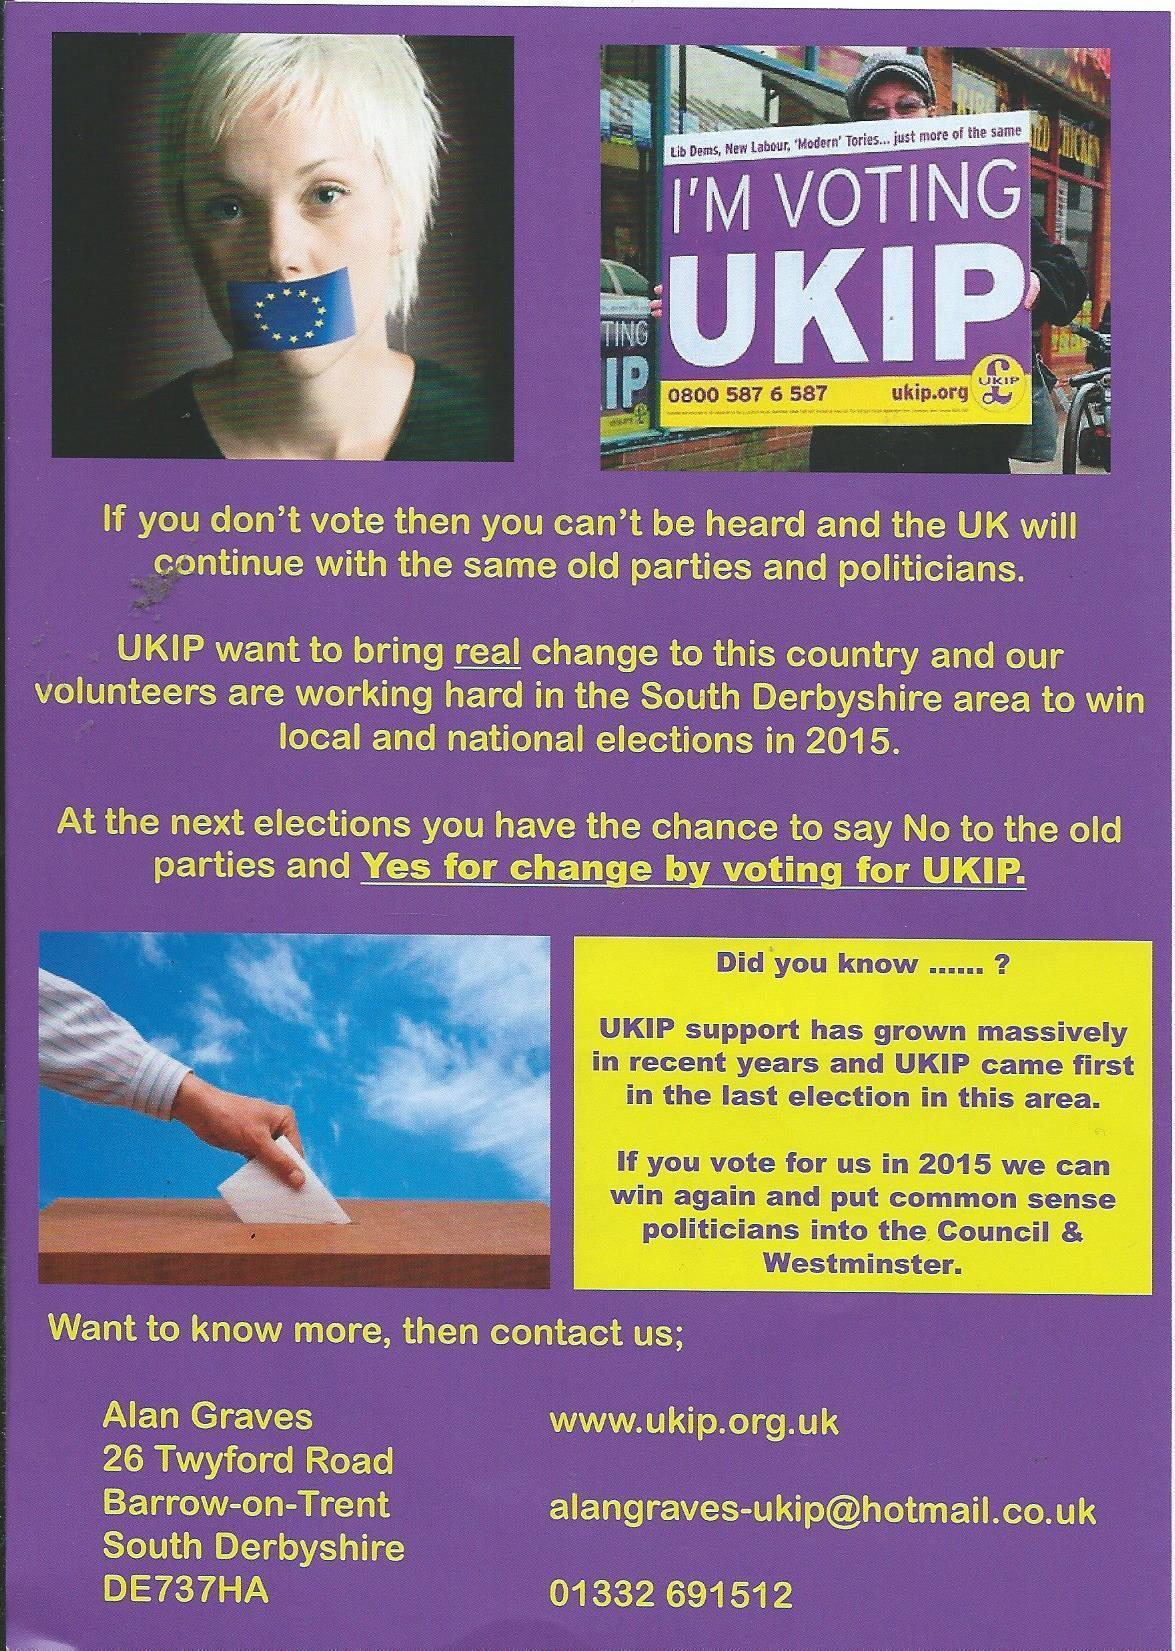
\includegraphics[width=0.3\textwidth]{28_1.jpg}
	\caption{}
	\label{fig:28_1}
\end{figure}

% Include the third image
\begin{figure}[H]
	\centering
	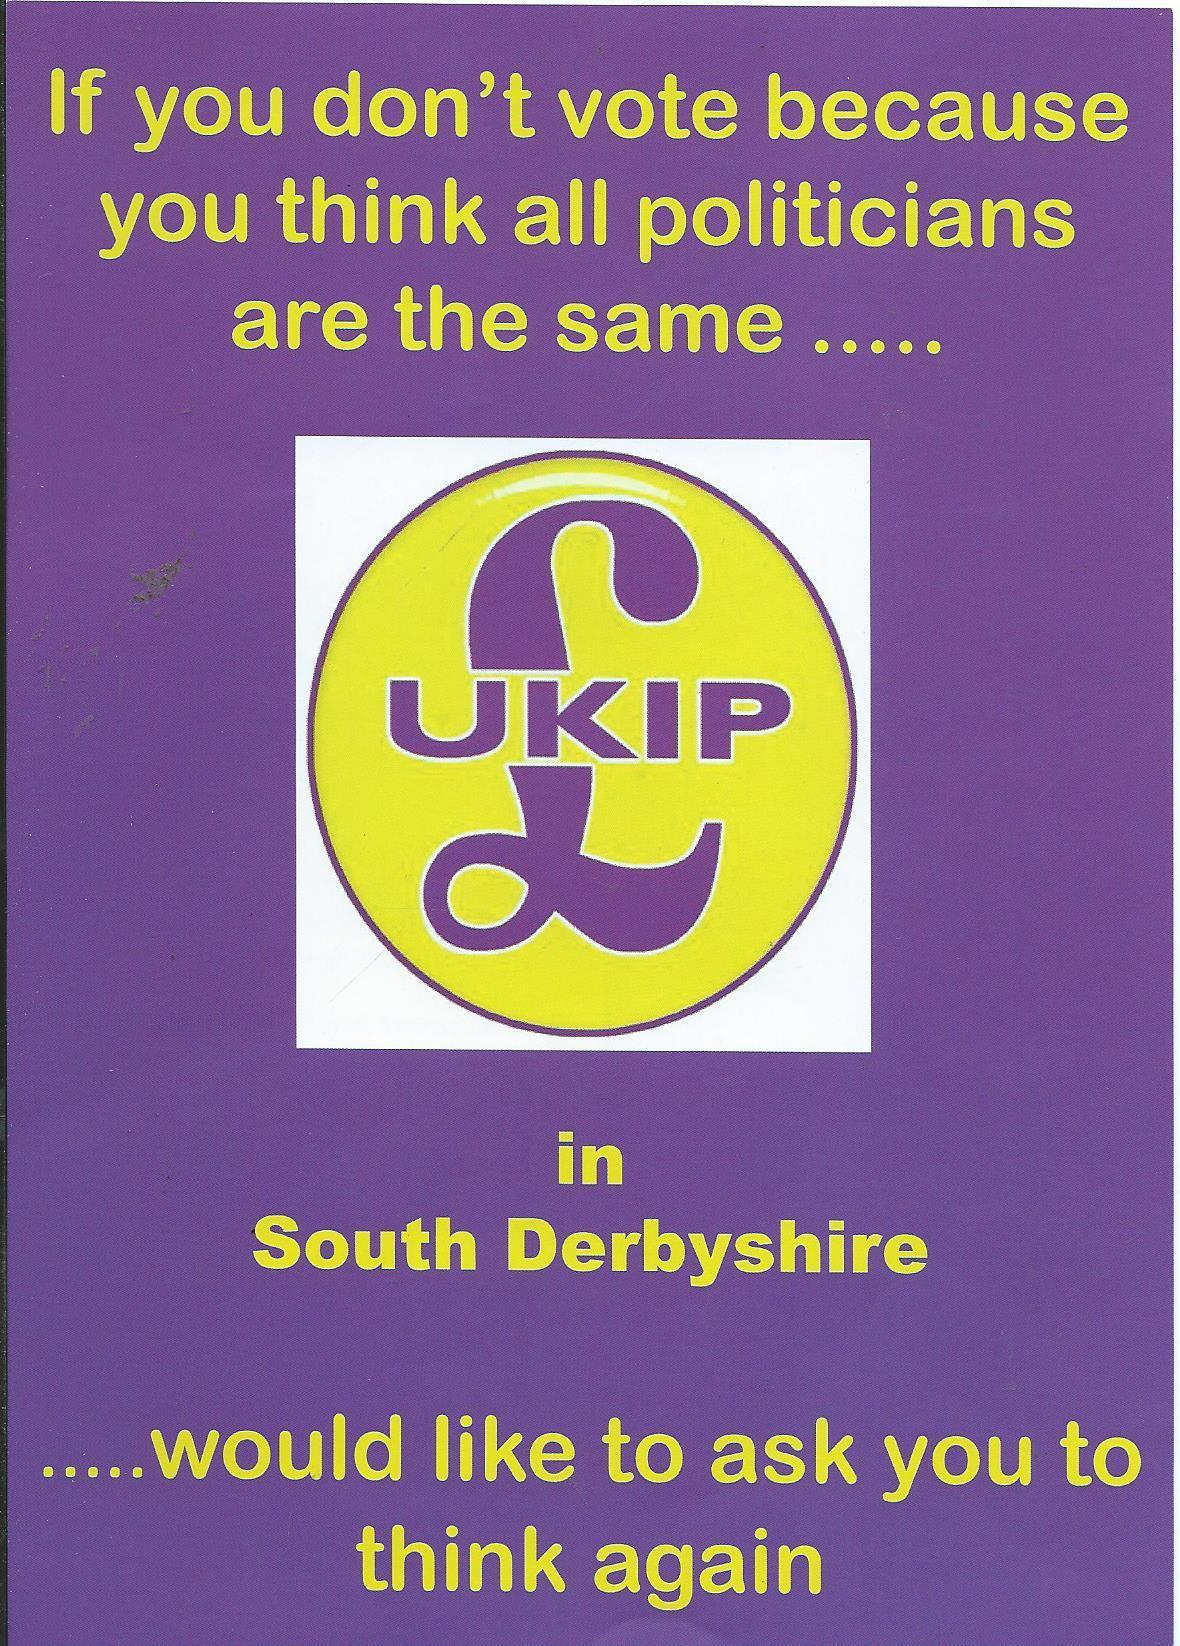
\includegraphics[width=0.3\textwidth]{28_2.jpg}
	\caption{}
	\label{fig:28_2}
\end{figure}





\subsection{Full Mean Environmental Mention Distribution Map}

\begin{figure}[H]
	\centering
	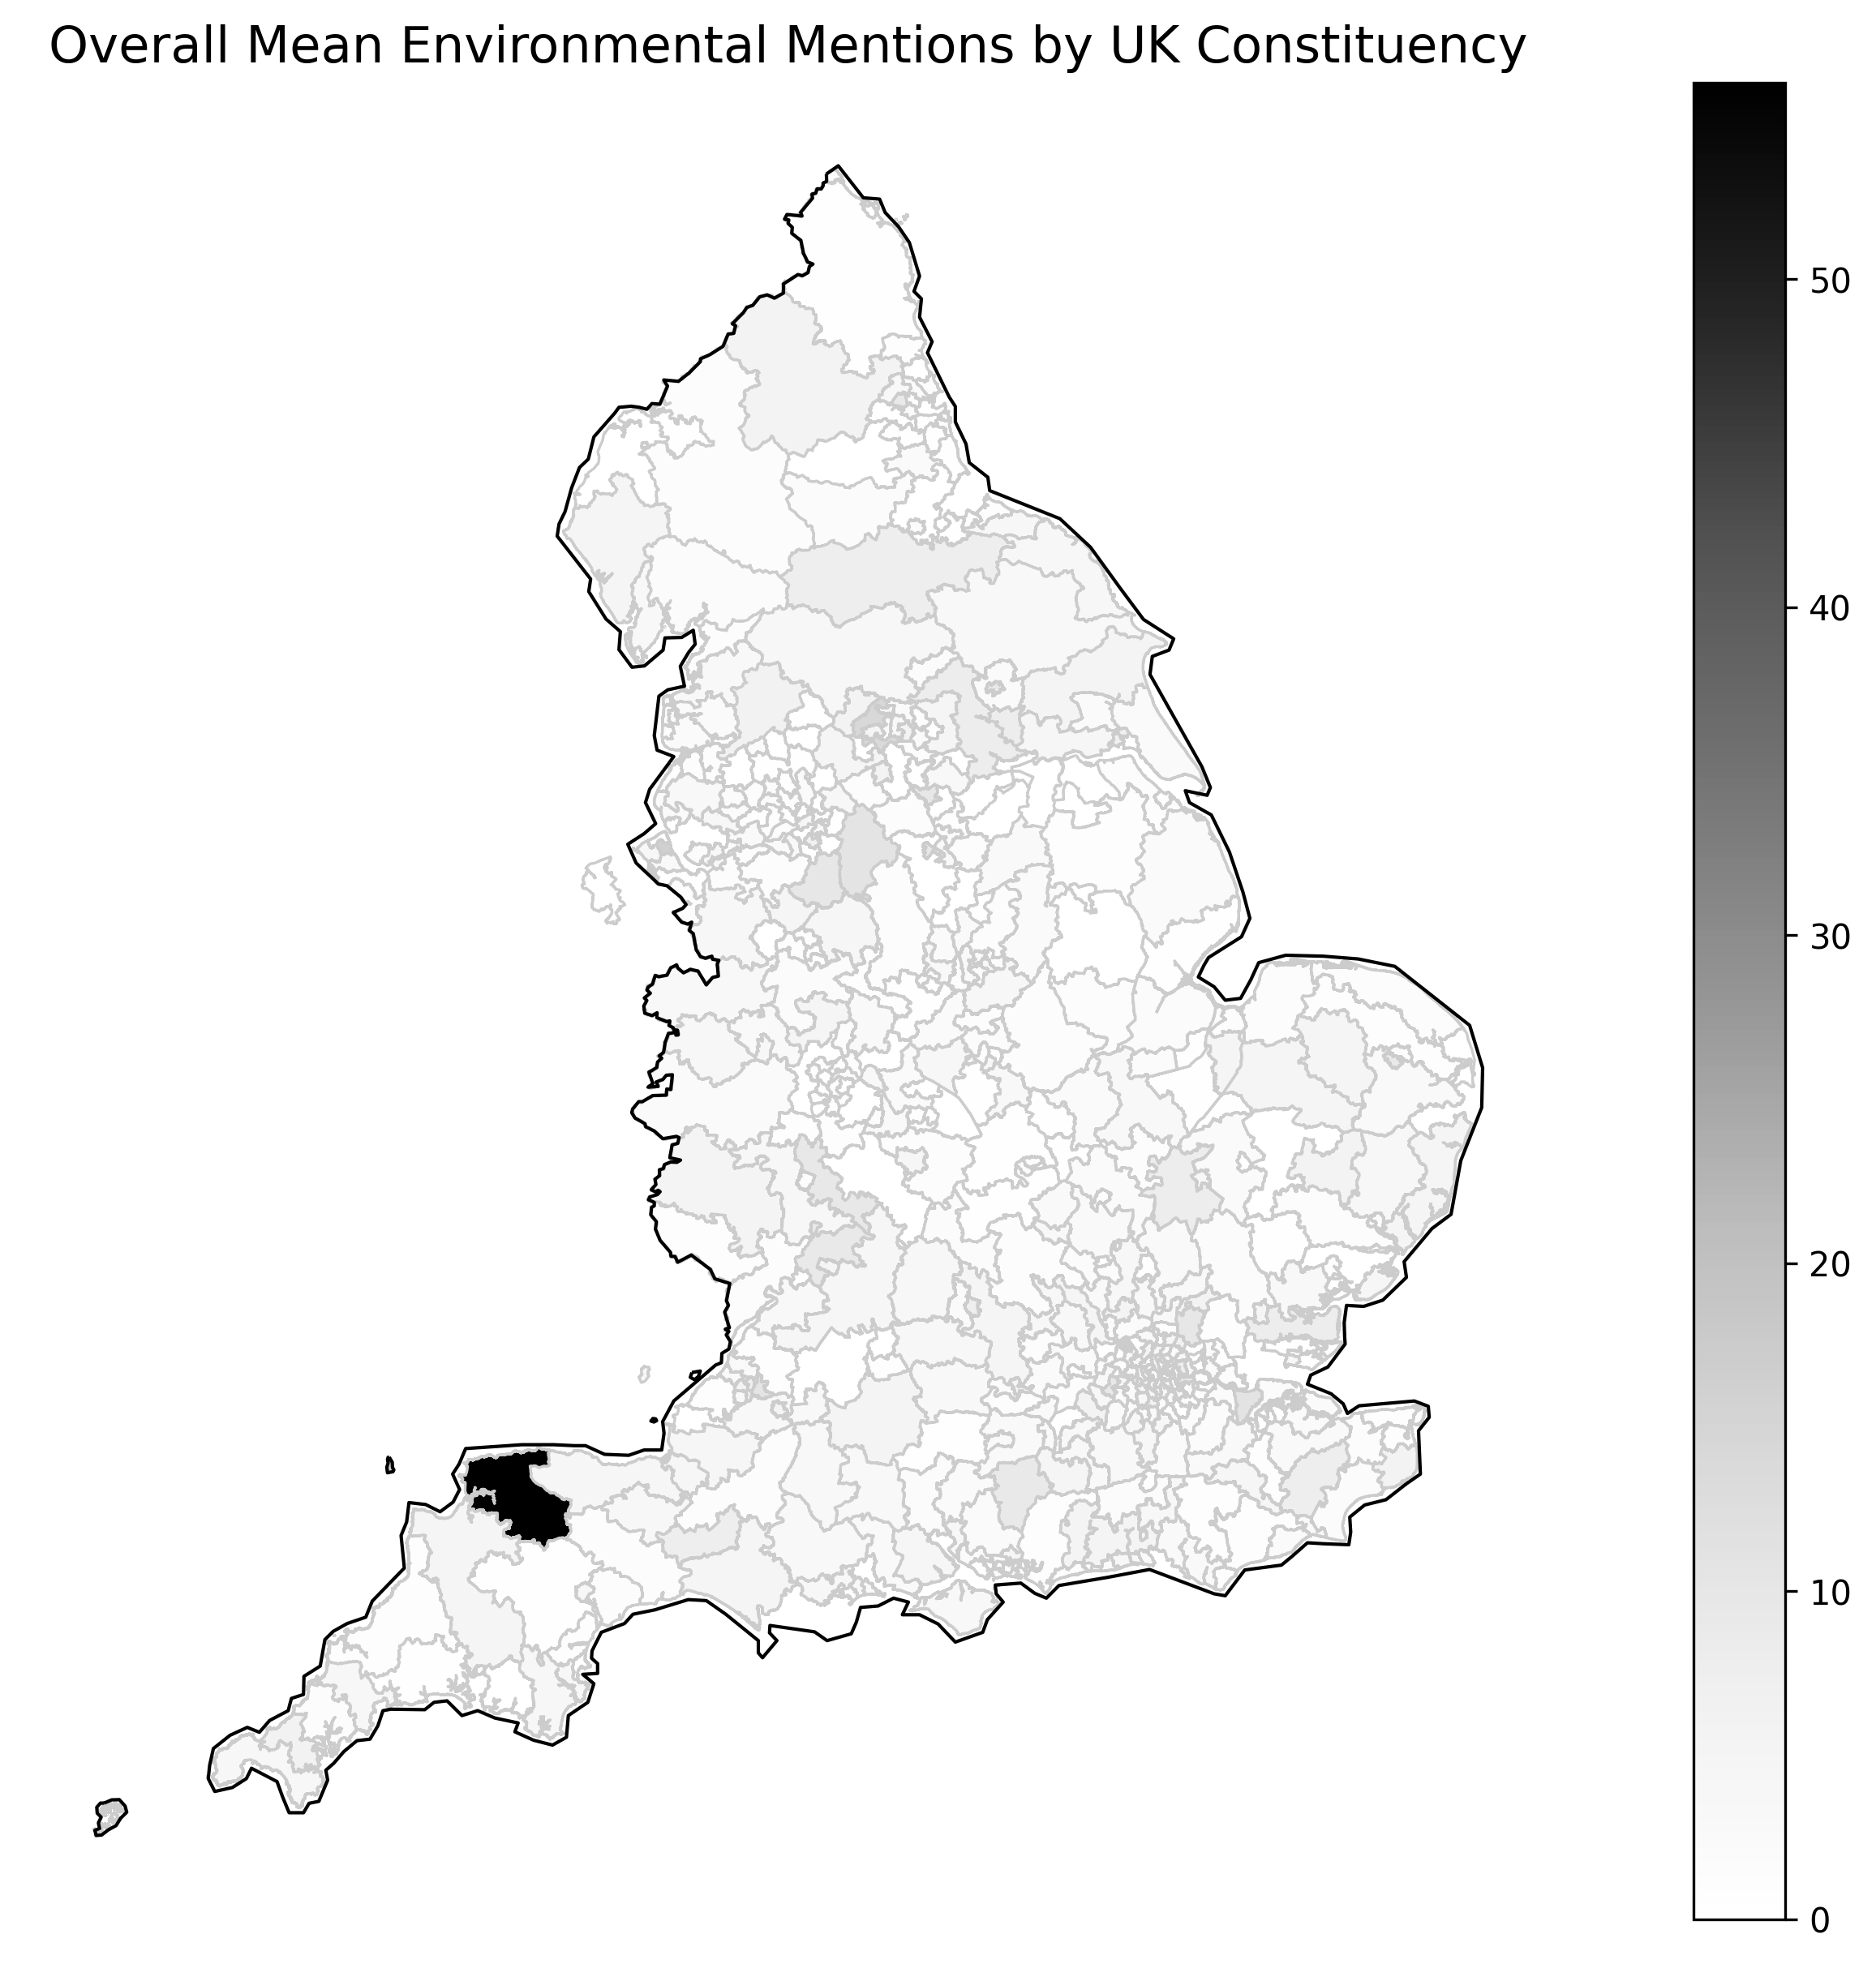
\includegraphics[width=0.38\textwidth]{plots/Overall_Environmental_Mentions.png}
	\caption{Mean Environmental Mentions By Constituency}
	\label{fig:meanenvbyconold}
\end{figure}





\end{document}
